\chapter{Cubed-sphere grids}
\label{chp-cs-grids}

The cubed-sphere grid was originally proposed by \citet{sadourny:1972} and was 
reinvestigated by \citet{ronchi:1996} and \citet{rancic:1996}. 
As is usual for Planotic grids, we start with a Platonic solid, in this case, a cube, 
which is circumscribed in a sphere. We then project its faces onto the sphere.
The original cubed-sphere, called the equidistant cubed-sphere, was proposed by 
\citet{sadourny:1972} but resulted in a non-uniform grid. 
To address this issue, a solution was proposed by introducing angular coordinates, 
leading to a quasi-uniform grid known as the equiangular cubed-sphere.
The cubed sphere consists of six panels, each one having a local Cartesian coordinate 
system. 
This makes it easier to extend methods from the plane to the sphere. 
In fact, \citet{putman:2007} extends the dimension splitting technique from 
\citet{lin:1996}, as presented in Chapter \ref{chp-2d-fv}, to the cubed-sphere.

There are essentially two major challenges when working with the cubed-sphere grid:
\begin{enumerate}
\item
The non-orthogonal grid system: This challenge is primarily related to the appearance of
metric terms in the equations. It adds computational cost and often requires conversions
between contravariant and covariant components of a velocity field.
\item
The discontinuity of the coordinate system at the cube edges: This is perhaps the most 
problematic challenge. Computing stencils along the cube edges becomes challenging due to 
the discontinuous nature of the coordinate system.
\end{enumerate}
One possible approach to compute stencils at the edges is to extend the local coordinate 
of each panel to its neighboring panels, adding ghost cells in the halo region. In the 
case of the equiangular cubed-sphere, ghost cell values lie on the same geodesics 
containing the data from the neighboring panels. This allows for the use of one-dimensional
high-order Lagrange interpolation to compute the stencils at the edges. 
This approach has been extensively used in the literature \citep{croisille:2013, 
katta:2015, katta:2015b, chen:2021} and was initially introduced by \citet{ronchi:1996}.
Alternatively, \citet{putman:2007} uses extrapolation for grid values near the cube edges.
Another approach that avoids the need for interpolation or extrapolation near the edges is 
the conformal cubed-sphere developed by \citet{rancic:1996}. While this grid leads to an 
orthogonal and continuous coordinate system near the edges, it generates grid singularities
near the cube corners, similar to the pole problem. 
An improved and more uniform conformal grid, called the Uniform Jacobian cubed sphere, was 
later proposed by \citet{rancic:2017}.
Each approach is likely to generate grid imprinting, and one of the goals of this work is 
to investigate the amount of grid imprinting produced by each method.

This chapter aims to review and investigated the geometrical properties
of the cubed-sphere. Besides that, we also aim to investigate the process
of interpolating/extrapolating near the cube edges.
We start with a basic review of the cubed-sphere mappings in Section \ref{cs-mappings},
while Section \ref{cs-halodata} investigates how we can apply 1D Lagrange interpolation using the adjacent panels
data to obtain values of a scalar/vector field on ghost cells, as well different edge
treatments when computing stencils near to the cube edges.
Final thoughts are presented in Section \ref{cs-conc}.

\section{Cubed-sphere mappings}
\label{cs-mappings}
\subsection{Equidistant cubed-sphere}
\label{equidistant-cs}
We start this chapter by introducing the equidistant cubed-sphere proposed by 
\citet{sadourny:1972}. Given $R>0$, we denote the sphere of radius $R$ 
centered at the origin of  $\mathbb{R}^3$ as:
\begin{equation*}
	\mathbb{S}^2_R = \{ P = (X,Y,Z) \in \mathbb{R}^3: X^2 + Y^2 + Z^2 = R^2\}.
\end{equation*}
We consider a parameter $a = \frac{R}{\sqrt{3}}$ representing the half-length of 
the cube, and the family of maps
$\Psi_{p}: [-a,a] \times [-a,a] \to \mathbb{S}^2_R$, $p=1, \ldots, 6$,
where:
\begin{equation*}
	\Psi_{1}(x,y) = \frac{R}{\sqrt{a^2 + x^2 + y^2}}(a, x, y), 
\end{equation*}
\begin{equation*}
	\Psi_{2}(x,y) = \frac{R}{\sqrt{a^2 + x^2 + y^2}}(-x, a, y), 
\end{equation*}
\begin{equation*}
	\Psi_{3}(x,y) = \frac{R}{\sqrt{a^2 + x^2 + y^2}}(-a, -x, y), 
\end{equation*}
\begin{equation*}
	\Psi_{4}(x,y) = \frac{R}{\sqrt{a^2 + x^2 + y^2}}(x, -a, y), 
\end{equation*}
\begin{equation*}
	\Psi_{5}(x,y) = \frac{R}{\sqrt{a^2 + x^2 + y^2}}(-y, x, a), 
\end{equation*}
\begin{equation*}
	\Psi_{6}(x,y) = \frac{R}{\sqrt{a^2 + x^2 + y^2}}(y, x, -a).
\end{equation*}
The set of 6 maps $\{\Psi_{p}, p = 1, \ldots, 6\}$ allow us to cover the sphere.
Here $p$ denotes a panel, and they are defined and orientated as Figure \ref{chp4-panels}
shows. Then, we can represent a point on the sphere using the cubed-sphere coordinates
$(x,y,p)$.

The derivative of the maps $\Psi_p$ are given by:
\begin{equation*}
	D\Psi_{1}(x,y) = \frac{R}{{(a^2 + x^2 + y^2)}^{3/2}}
	\begin{bmatrix}
		-ax & -ay \\
	 	 a^2+y^2  & -xy \\
		 -xy  & a^2+x^2
	\end{bmatrix},
\end{equation*}
\begin{equation*}
	D\Psi_{2}(x,y) = \frac{R}{{(a^2 + x^2 + y^2)}^{3/2}}
	\begin{bmatrix}
		-(a^2+y^2) & xy \\
		 -ax &  -ay \\
		 -xy &  a^2+x^2
	\end{bmatrix},
\end{equation*}
\begin{equation*}
	D\Psi_{3}(x,y) = \frac{R}{{(a^2 + x^2 + y^2)}^{3/2}}
	\begin{bmatrix}
		 ax &  ay \\
		-(a^2+y^2) & xy \\
		 -xy &  a^2+x^2
	\end{bmatrix},
\end{equation*}
\begin{equation*}
	D\Psi_{4}(x,y) = \frac{R}{{(a^2 + x^2 + y^2)}^{3/2}}	
	\begin{bmatrix}
		 a^2+y^2 &  -xy \\
		 ax & ay \\
		 -xy &  a^2+x^2
	\end{bmatrix},
\end{equation*}
\begin{equation*}
	D\Psi_{5}(x,y) = \frac{R}{{(a^2 + x^2 + y^2)}^{3/2}}	
	\begin{bmatrix}
		 xy  & -(a^2+x^2) \\
	 	 a^2+y^2  &  -xy \\
		-ax & -ay
	\end{bmatrix},
\end{equation*}
\begin{equation*}
	D\Psi_{6}(x,y) = \frac{R}{{(a^2 + x^2 + y^2)}^{3/2}}
	\begin{bmatrix}
		 -xy  &  a^2+x^2 \\
		 a^2+y^2  &  -xy \\
		 ax &  ay
	\end{bmatrix}.
\end{equation*}
With the aid of the derivative, we may define a basis of tangent vectors 
$\{ \boldsymbol{g}_{x}, \boldsymbol{g}_{y} \}$ on each point on the sphere by:
\begin{equation*}
	\boldsymbol{g}_{x}(x,y,p) = D\Psi_{p}(x,y)
	\begin{bmatrix}
		 1 \\
		 0
	\end{bmatrix},
	\boldsymbol{g}_{y}(x,y,p) = D\Psi_{p}(x,y)
	\begin{bmatrix}
		 0 \\
		 1
	\end{bmatrix}.
\end{equation*}
Notice that
\begin{equation*}
	\label{chp3-eqdistant-psitensor}
	[D\Psi_{p}(x,y)]^TD\Psi_{p}(x,y)
	= \frac{R^2}{(a^2 + x^2 + y^2)^2}
	\begin{bmatrix}
		 a^2 + x^2 &  -xy \\
		 -xy & a^2 + y^2
	\end{bmatrix},
\end{equation*}
does not depend on $p$.
Hence, it makes sense to define the matrix 
$G_{\Psi}(x,y) = [D\Psi_{p}(x,y)]^TD\Psi_{p}(x,y)$ 
which is known as metric tensor.
It is easy to see that:
\begin{equation*}
	\label{chp3-eqdistant-psi-metric-tensor}
	G_{\Psi}(x,y) = 
	\begin{bmatrix}
		\langle \boldsymbol{g}_{x}(x,y,p), \boldsymbol{g}_{x}(x,y,p) \rangle & 
		\langle \boldsymbol{g}_{x}(x,y,p), \boldsymbol{g}_{y}(x,y,p) \rangle \\
		\langle \boldsymbol{g}_{x}(x,y,p), \boldsymbol{g}_{y}(x,y,p) \rangle  &
		\langle \boldsymbol{g}_{y}(x,y,p), \boldsymbol{g}_{y}(x,y,p) \rangle 
	\end{bmatrix},
\end{equation*}
where $\langle \cdot, \cdot \rangle$ denotes 
the standard inner product of $\mathbb{R}^3$,
and that $G_{\Psi}(x,y)$ is positive-definite, 
$\forall (x,y) \in [-a,a]\times[-a,a]$.
The Jacobian of the metric tensor $G_{\Psi}(x,y)$ is then given by:
\begin{equation*}
	\sqrt{|\det{G_{\Psi}(x,y)}|} = \frac{R^2}{(a^2+x^2+y^2)^{3/2}}a.
\end{equation*}
\begin{figure}[!htb]
	\centering
		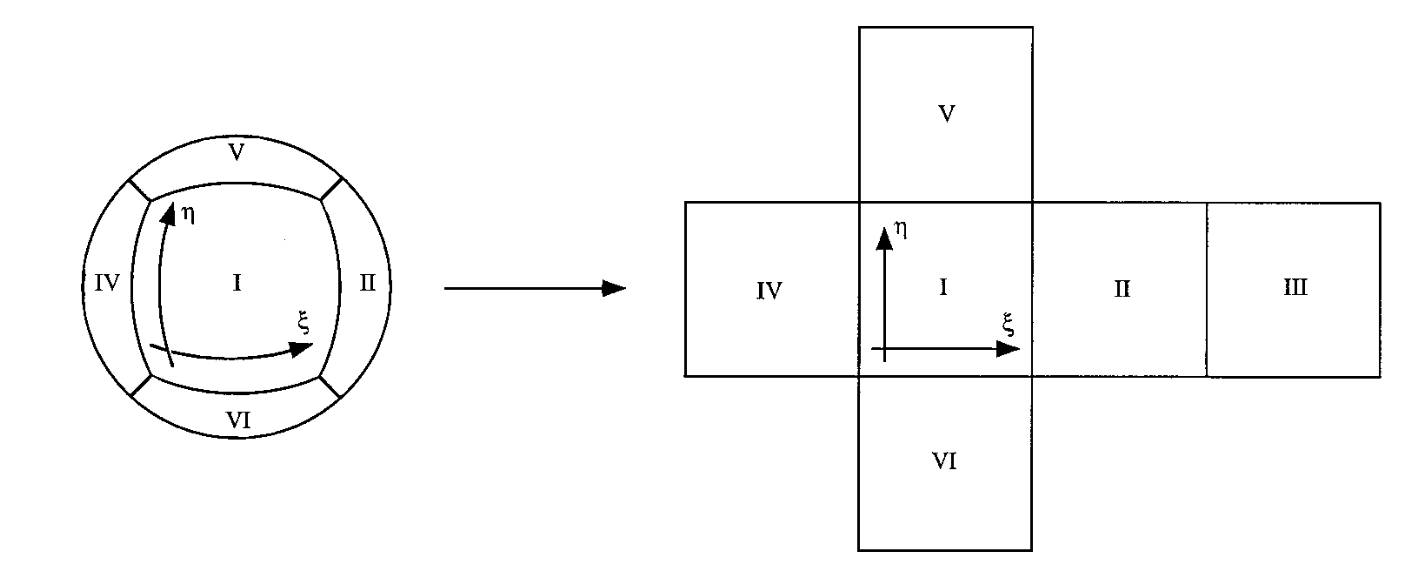
\includegraphics[width=0.8\linewidth]{chp4_panels}
	\caption{Cubed-sphere panels definition and orientation.
    Figure taken from \citet{jung:2019}.\label{chp4-panels}}
\end{figure}

\subsection{Equiangular cubed-sphere}
\label{equiangular-cs}
Another cubed-sphere mapping is the equiangular mapping \citep{ronchi:1996},
which leads to a more uniform grid.
This mapping is a composition of equidistant mapping with angular coordinates.
We consider again $a=\frac{R}{\sqrt{3}}$ and we define the family of maps
$\Phi_{p}: [-\frac{\pi}{4},\frac{\pi}{4}]  \times [-\frac{\pi}{4},\frac{\pi}{4}] 
\to \mathbb{S}^2_R$, $p=1, \ldots, 6$, given by $\Phi_{p}(x,y) = \Psi_{p}(a\tan{x},
a\tan{y})$.
The coordinates $(a\tan{x}, a\tan{y})$ are called angular coordinates.
By the chain rule:
\begin{equation*}
	D\Phi_{p}(x,y) = a
	D\Psi_{p}(a\tan{x}, a\tan{y})
	\begin{bmatrix}
		\frac{1}{\cos^2 x} & 0 \\ 
		0 & \frac{1}{\cos^2 y} 
	\end{bmatrix},
\end{equation*}
and therefore we can define the following tangent vectors
\begin{align}
    \label{chp4-tgvectors}
	\boldsymbol{r}_{x}(x,y,p) = D\Phi_{p}(x,y)
	\begin{bmatrix}
		 1 \\
		 0
	\end{bmatrix}
	= \frac{a}{\cos^2 x}
	\boldsymbol{g}_{x}(\tan{x}, \tan{y}, p)
	,\\
	\boldsymbol{r}_{y}(x, y ,p) = D\Phi_{p}(x,y)
	\begin{bmatrix}
		 0 \\
		 1
	\end{bmatrix}
	= \frac{a}{\cos^2 y}
	\boldsymbol{g}_{y}(\tan{x}, \tan{y}, p),
\end{align}
Again, it makes sense to define the matrix 
\begin{align*}
	G_{\Phi}(x,y) &= [D\Phi_{p}(x,y)]^TD\Phi_{p}(x,y) \\
	&= a^2
	[D\Psi_{p}(a\tan{x},a\tan{y})]^T
	\begin{bmatrix}
		\frac{1}{\cos^4 x} & 0 \\ 
		0 & \frac{1}{\cos^4 y} 
	\end{bmatrix}
	D\Psi_{p}(a\tan{x}, a\tan{y}),
\end{align*}
that does not depend on $p$ and is the  metric tensor.
It is easy to see that:
\begin{equation}
	\label{chp3-eqangle-phi-metric-tensor}
	G_{\Phi}(x,y) = 
	\begin{bmatrix}
		\langle \boldsymbol{r}_{x}(x,y,p), \boldsymbol{r}_{x}(x,y,p) \rangle & 
		\langle \boldsymbol{r}_{x}(x,y,p), \boldsymbol{r}_{y}(x,y,p) \rangle \\
		\langle \boldsymbol{r}_{x}(x,y,p), \boldsymbol{r}_{y}(x,y,p) \rangle  &
		\langle \boldsymbol{r}_{y}(x,y,p), \boldsymbol{r}_{y}(x,y,p) \rangle 
	\end{bmatrix},
\end{equation}
and that $G_{\Phi}(x,y)$ is positive-definite, 
$\forall (x,y) \in [-\frac{\pi}{4},\frac{\pi}{4}] 
\times [-\frac{\pi}{4},\frac{\pi}{4}]$.
The Jacobian of the metric tensor $G_{\Phi}(x,y)$ is then given by:
\begin{align}
	\label{metrictensor-cs-equiangular}
	\begin{split}
		\sqrt{|\det{G_{\Phi}(x,y)}|} &= \frac{a}{\cos^2 x \cos^2 y}
		\frac{R^2}{(a^2 + a^2\tan^2x + a^2\tan^2y)^{3/2}}a\\
		&= \frac{R^2}{\cos^2 x \cos^2 y}
		\frac{1}{(1 + \tan^2x + \tan^2y)^{3/2}}.
	\end{split}
\end{align}

\subsection{Tangent vectors on the sphere}
\label{cs-tgvectors}
The tangent space at $P \in \mathbb{S}^2_R$ is denoted by $T_P \mathbb{S}^2$.
It is easy to see that:
\begin{equation*}
	T_P\mathbb{S}^2_R = \{P_0 \in \mathbb{R}^3: \langle P,P_0\rangle = 0\}.
\end{equation*}
We are going to consider three ways to represent an element of $\mathbb{S}_R^2$:
using $(X,Y,Z)$ coordinates, or using $(\lambda, \phi)$
latitude-longitude coordinates, or, at last, using the cubed-sphere
coordinates $(x,y,p)$, where $(x,y)$ are the cube face coordinates and 
$p \in \{1,2,\cdots, 6\}$ stands for a cube panel.
We say that a vector field $\boldsymbol{u}: \mathbb{S}^2_R \to 
\mathbb{R}^3$ is tangent on  the sphere if
$\boldsymbol{u}(P) \in T_P\mathbb{S}^2_R$, $\forall P \in \mathbb{S}^2_R$.

\subsubsection{Conversions between latitude-longitude and contravariant coordinates}
\label{anexo-sph-ll}
We consider the latitude-longitude mapping 
$\Psi_{ll}: [0,2\pi] \times [-\frac{\pi}{2},\frac{\pi}{2}] \to \mathbb{S}^2_R$, given by:
\begin{align}
	\label{ll2sph}
	X(\lambda,\phi) &= R\cos \phi \cos \lambda,\\
	Y(\lambda,\phi) &= R\cos \phi \sin \lambda,\\
	Z(\lambda,\phi) &= R\sin \phi.
\end{align}
The derivative or Jacobian matrix of the mapping $\Psi_{ll}$ is given by:
\begin{equation}
	\label{dpsi}
	D\Psi_{ll} (\lambda,\phi) = 
	R \begin{bmatrix}
		  -\cos \phi \sin \lambda &  -\sin \phi \cos \lambda \\
		   \cos \phi \cos \lambda & \sin \phi \sin \lambda \\
		  0  &  \cos \phi
	\end{bmatrix}.
\end{equation}
Using this matrix columns, we can define the tangent vectors:
\begin{equation}
	\boldsymbol{r}_{\lambda}(\lambda,\phi) = D\Psi_{ll}(\lambda,\phi)
	\begin{bmatrix}
		 1 \\
		 0
	\end{bmatrix}, \quad
	\boldsymbol{r}_{\phi}(\lambda,\phi) = D\Psi_{ll}(\lambda,\phi)
	\begin{bmatrix}
		 0 \\
		 1
	\end{bmatrix}.
\end{equation}
We normalize the vectors $\boldsymbol{r}_\lambda$ and $\boldsymbol{r}_\phi$
and we obtain unit tangent vectors on the sphere at $\Phi_{ll}(\lambda, \phi)$:
\begin{equation}
	\label{latlon_tg_vectors}
	\boldsymbol{e}_{\lambda}(\lambda,\phi) = 
	\begin{bmatrix}
		 -\sin \lambda \\
		  \cos \lambda \\
		  0
	\end{bmatrix}, \quad
	\boldsymbol{e}_{\phi}(\lambda,\phi) =
	\begin{bmatrix}
		 -\sin \phi \cos \lambda \\
		 -\sin \phi \sin \lambda \\
			  \cos \phi
	\end{bmatrix}.
\end{equation}
Let us consider a tangent vector field $\boldsymbol{u}: \mathbb{S}^2_R \to 
\mathbb{R}^3$ on the sphere, represented as
\begin{equation}
	\label{latlon-wind}
	\boldsymbol{u}(\lambda, \phi) = 
    u_{\lambda} (\lambda, \phi) \boldsymbol{e}_{\lambda} (\lambda, \phi) + 
	v_{\phi} (\lambda, \phi) \boldsymbol{e}_{\phi} (\lambda, \phi). 
\end{equation}
Or, we may also represent this vector field using the basis 
obtained by cubed-sphere coordinates:
\begin{equation}
	\label{contravariant-wind}
	\boldsymbol{u}(x, y, p) = 
	{u}(x, y, p) \boldsymbol{r}_{x}(x, y, p) + 
	{v}(x, y, p) \boldsymbol{r}_{y}(x, y, p).
\end{equation}
This representation is known as contravariant representation.
In order to relate the latitude-longitude representation
with the contravariant representation, we notice that:
\begin{align}
	\label{basis-convertion1}
	\boldsymbol{r}_x(x, y, p) &= 
	\langle \boldsymbol{r}_{x} , \boldsymbol{e}_{\lambda}\rangle
	\boldsymbol{e}_{\lambda} (\lambda, \phi)  
	+ \langle \boldsymbol{r}_{x} , \boldsymbol{e}_{\phi}\rangle
	\boldsymbol{e}_{\phi} (\lambda, \phi), \\
	\label{basis-convertion2}
	\boldsymbol{r}_y(x, y, p) &=  
	\langle \boldsymbol{r}_{y} , \boldsymbol{e}_{\lambda}\rangle
	  \boldsymbol{e}_{\lambda} (\lambda, \phi) 
	+ \langle \boldsymbol{r}_{y} , \boldsymbol{e}_{\phi}\rangle
	\boldsymbol{e}_{\phi} (\lambda, \phi), 
\end{align}
which holds since the vectors $\boldsymbol{e}_{\lambda}(\lambda, \phi)$ and
$\boldsymbol{e}_{\phi}(\lambda, \phi)$ are orthogonal.
Replacing Equations \eqref{basis-convertion1} and \eqref{basis-convertion2}
in Equation \eqref{contravariant-wind}, we obtain the values $(u_\lambda, v_\phi)$
in terms of the contravariant components $({u},{v})$ 
as the following matrix equation:
\begin{equation}
	\label{ll-to-contravariant}
	\begin{bmatrix}
		 u_\lambda (\lambda, \phi) \\
		 v_\phi (\lambda, \phi) 
	\end{bmatrix}
	=
	\begin{bmatrix}
		\langle \boldsymbol{r}_x, \boldsymbol{e}_\lambda \rangle 
		& \langle \boldsymbol{r}_y, \boldsymbol{e}_\lambda \rangle \\
		\langle \boldsymbol{r}_x, \boldsymbol{e}_\phi \rangle 
		& \langle \boldsymbol{r}_y, \boldsymbol{e}_\phi \rangle \\
	\end{bmatrix}
	\begin{bmatrix}
		{u}(x,y,p) \\
		{v}(x,y,p)
	\end{bmatrix}.
\end{equation}
Conversely, we may express the contravariant components in terms of
latitude-longitude components by inverting Equation \eqref{ll-to-contravariant}:
\begin{equation}
	\label{contravariant-to-ll}
	\begin{bmatrix}
		{u}(x,y,p) \\
		{v}(x,y,p)
	\end{bmatrix}
	=
	\frac{1}{\langle \boldsymbol{r}_x, \boldsymbol{e}_\lambda\rangle
	\langle \boldsymbol{r}_y, \boldsymbol{e}_\phi \rangle
	-\langle \boldsymbol{r}_y, \boldsymbol{e}_\lambda \rangle
	\langle \boldsymbol{r}_x, \boldsymbol{e}_\phi \rangle}
	\begin{bmatrix}
		  \langle \boldsymbol{r}_y, \boldsymbol{e}_\phi \rangle 
		&-\langle \boldsymbol{r}_y, \boldsymbol{e}_\lambda \rangle \\
		 -\langle \boldsymbol{r}_x, \boldsymbol{e}_\phi \rangle 
		& \langle \boldsymbol{r}_x, \boldsymbol{e}_\lambda \rangle \\
	\end{bmatrix}
	\begin{bmatrix}
		 u_\lambda (\lambda, \phi) \\
		 v_\phi (\lambda, \phi) 
	\end{bmatrix}.
\end{equation}

\subsubsection{Covariant/contravariant conversion}
\label{anexo-cov-con}
Let us consider again a tangent vector field $\boldsymbol{u}: \mathbb{S}^2_R \to 
\mathbb{R}^3$ on the sphere. Its contravariant representation 
is given by Equation \eqref{contravariant-wind}.
The covariant components $(U,V)$ are given by:
\begin{align}
	\label{covariant-u}
	U(x,y,p) = \langle \boldsymbol{u}(x,y,p) , \boldsymbol{r}_x(x,y,p)  \rangle, \\
	\label{covariant-v}
	V(x,y,p) = \langle \boldsymbol{u}(x,y,p) , \boldsymbol{r}_y(x,y,p)  \rangle.
\end{align}
Replacing Equation \eqref{contravariant-wind} in 
Equations \eqref{covariant-u} and \eqref{covariant-v} we obtain
the relation covariant components in terms of the
contravariant terms:
\begin{equation}
	\label{contravariant-to-covariant}
	\begin{bmatrix}
		{U}(x,y,p) \\
		{V}(x,y,p)
	\end{bmatrix}
	=
	\begin{bmatrix}
		  \langle \boldsymbol{r}_x, \boldsymbol{r}_x \rangle
		& \langle \boldsymbol{r}_x, \boldsymbol{r}_y \rangle \\
		  \langle \boldsymbol{r}_x, \boldsymbol{r}_y \rangle 
		& \langle \boldsymbol{r}_y, \boldsymbol{r}_y \rangle \\
	\end{bmatrix}
	\begin{bmatrix}
		{u} (x,y,p) \\
		{v} (x,y,p) 
	\end{bmatrix}.
\end{equation}
We may express the contravariant components in terms of 
the covariant terms inverting Equation \eqref{contravariant-to-covariant}:
\begin{equation}
	\label{convariant-to-contravariant}
	\begin{bmatrix}
		{u}(x,y,p) \\
		{v}(x,y,p)
	\end{bmatrix}
	= \frac{1}{\langle \boldsymbol{r}_x, \boldsymbol{r}_x \rangle
               \langle \boldsymbol{r}_y, \boldsymbol{r}_y \rangle
             - \langle \boldsymbol{r}_x, \boldsymbol{r}_y \rangle^2}
	\begin{bmatrix}
		  \langle \boldsymbol{r}_y, \boldsymbol{r}_y \rangle
		& -\langle \boldsymbol{r}_x, \boldsymbol{r}_y \rangle \\
		  -\langle \boldsymbol{r}_x, \boldsymbol{r}_y \rangle 
		& \langle \boldsymbol{r}_x, \boldsymbol{r}_x \rangle \\
	\end{bmatrix}
	\begin{bmatrix}
		{U} (x,y,p) \\
		{V} (x,y,p) 
	\end{bmatrix}.
\end{equation}
Notice that combining Equations \eqref{contravariant-to-covariant}
and \eqref{convariant-to-contravariant} with Equations 
\eqref{ll-to-contravariant} and \eqref{contravariant-to-ll}
one may get relations between the latitude-longitude 
components and the covariant components.

\subsection{Notation}
\label{cs-notation}
Let us denote by $\Sigma_p: \Omega \to \mathbb{S}^2_R$, $p=1,\ldots,6$, $\Omega=[-a,a]^2$,
a cubed-sphere mapping like the equiangular or the equidistant mappings introduced in
Section \ref{cs-mappings}.
With these mappings, we denote by ${\boldsymbol{r}_x(x,y,p),\boldsymbol{r}_y(x,y,p)}$
the basis of tangent vectors at $(x,y,p)$.
The metric tensor is denoted by $\sigma(x,y) =\sqrt{|\det{G_{\Sigma}(x,y,p)}|}$, where
\begin{equation}
	\label{chp3-sigma-metric-tensor}
	G_{\Sigma}(x,y,p) = 
	\begin{bmatrix}
		\langle \boldsymbol{r}_{x}(x,y,p), \boldsymbol{r}_{x}(x,y,p) \rangle & 
		\langle \boldsymbol{r}_{x}(x,y,p), \boldsymbol{r}_{y}(x,y,p) \rangle \\
		\langle \boldsymbol{r}_{x}(x,y,p), \boldsymbol{r}_{y}(x,y,p) \rangle  &
		\langle \boldsymbol{r}_{y}(x,y,p), \boldsymbol{r}_{y}(x,y,p) \rangle 
	\end{bmatrix}.
\end{equation}
We will utilize the notation introduced in Section \ref{chp3-sec-not} throughout this chapter.
The parameter $\nu$ represents a non-negative integer indicating the number of ghost cell layers in each panel boundary, called halo size.

To introduce the cubed-sphere, we consider a $(\Delta x, \Delta y)$-grid denoted by 
$\Omega_{\Delta x, \Delta y} = (\Omega_{ij})_{i,j=-\nu+1,\ldots,N+\nu}$, 
where $\Delta x = \Delta y$, and it covers the domain $\Omega$. 
A control volume of the cubed-sphere is denoted by $\Omega_{ijp}$, defined as follows:
\begin{equation*}
	\Omega_{ijp} = \Sigma_p(\Omega_{ij})
	\quad -\nu+1 \leq i, j \leq N+\nu, \quad 1 \leq p \leq 6.
\end{equation*}
The cubed-sphere grid refers to the collection of control volumes 
$(\Omega_{ijp})_{i,j=-\nu+1,\ldots,N+\nu}^{p=1,\ldots,6}$. 
In Figure \ref{chp4-cs-grid}, an example of the cubed-sphere grid is depicted,
excluding the ghost cells. This grid is generated using the equidistant and equiangular mappings for $N=20$.
\begin{figure}[!htb]
	\centering
	\begin{subfigure}{0.48\textwidth}
		\centering
		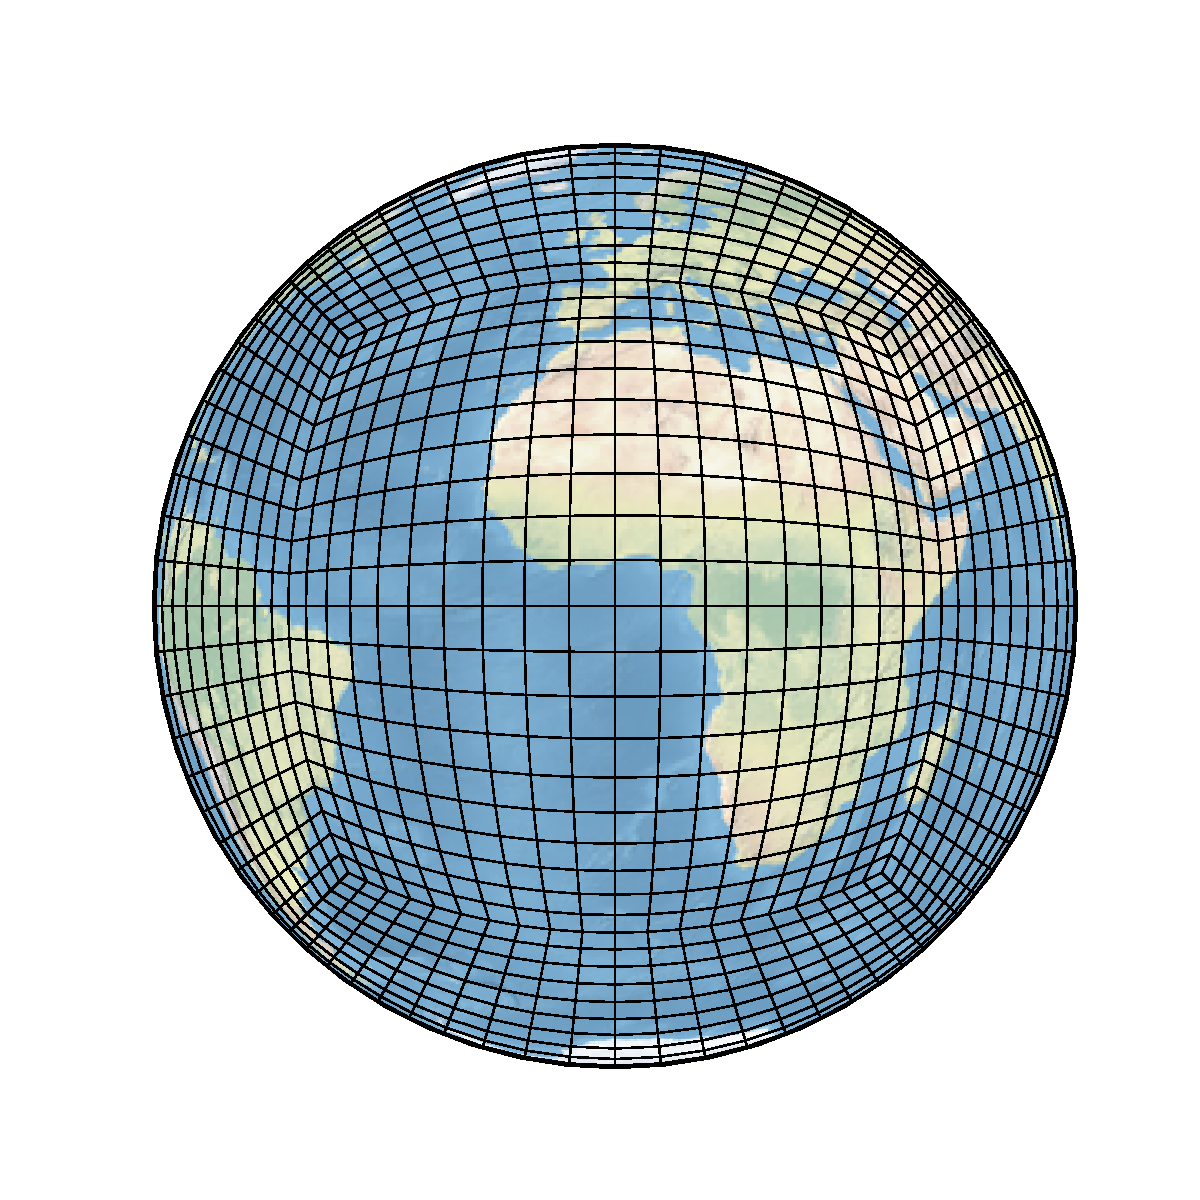
\includegraphics[width=1\linewidth]{gnomonic_equidistant_20_sphere}
		\caption{Equidistant}
	\end{subfigure}
	\begin{subfigure}{0.48\textwidth}
		\centering
		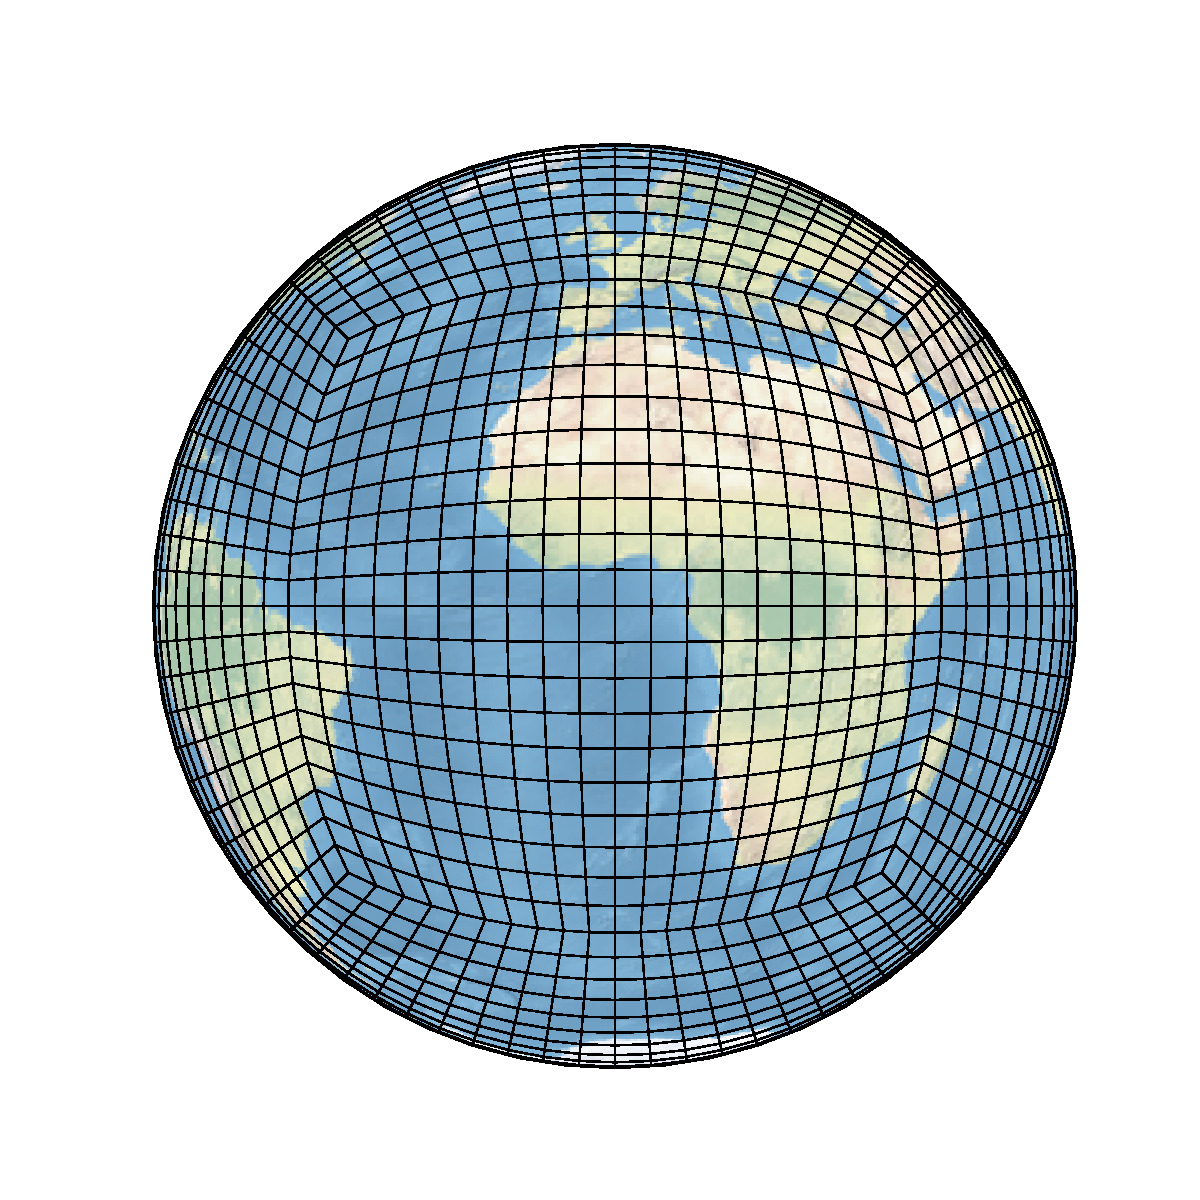
\includegraphics[width=1\linewidth]{gnomonic_equiangular_20_sphere}
		\caption{Equiangular}
	\end{subfigure}
	\caption{Equidistant (a) and equiangular (b) cubed-spheres generated with $N=20$.
		\label{chp4-cs-grid}}
\end{figure}

From Figure \ref{chp4-cs-grid}, it is evident that the equiangular cubed-sphere
exhibits a higher degree of uniformity compared to the equidistant cubed-sphere.
As noted by \citet{rancic:1996}, the ratio between the maximum and minimum cell
areas on the equiangular cubed-sphere is approximately 1.3,
whereas the same ratio is approximately 5.2 on the equidistant cubed-sphere. 

We also utilize the notation $\mathcal{CS}_N=\mathbb{R}^{(N+\nu)\times(N+\nu)\times 6}$
to represent grid functions on the cubed-sphere at cell centers.
Let's assume we have a function $q:\mathbb{S}^2_R\times[0,T] \to \mathbb{R}$, 
and we have a $(\Delta x, \Delta y, \Delta t, \lambda)$-discretization of $\Omega \times [0,T]$.
We introduce $q^n \in \mathcal{CS}^N$, which represents the grid function $q$
evaluated at the discrete points. 
In other words, $q^n_{ijp} = q(x_i,y_j,p,t^n)$, where $i,j=-\nu +1, \ldots, N+\nu$, and $p=1, \ldots, 6$.
Furthermore, we use the notations $q^n_{i+\frac{1}{2},j,p} = q(x_{i+\frac{1}{2}},y_j, t^n)$ 
for $i=-\nu, \ldots, N+\nu$ and $j=-\nu +1, \ldots, N+\nu$ to represent $q$ at the midpoint of edges in
the $x$ direction.
Similarly, we use $q^n_{i,j+\frac{1}{2},p} = q(x_i,y_{j+\frac{1}{2}},t^n)$ for $i=-\nu +1, \ldots, N+\nu$ and $j=-\nu, \ldots, N+\nu$ to represent $q$ at the midpoint of edges in the $y$ direction.
When $q$ does not depend on the time variable $t$, we can omit the index $n$.
In Figure \ref{chp4-cs-grid-function}, we depict a grid function at centers, edge midpoints in the $x$ direction
and edge midpoints in the $y$ direction for the equiangular cubed-sphere considering
the halo size equal to three.
\begin{figure}[!htb]
	\centering
	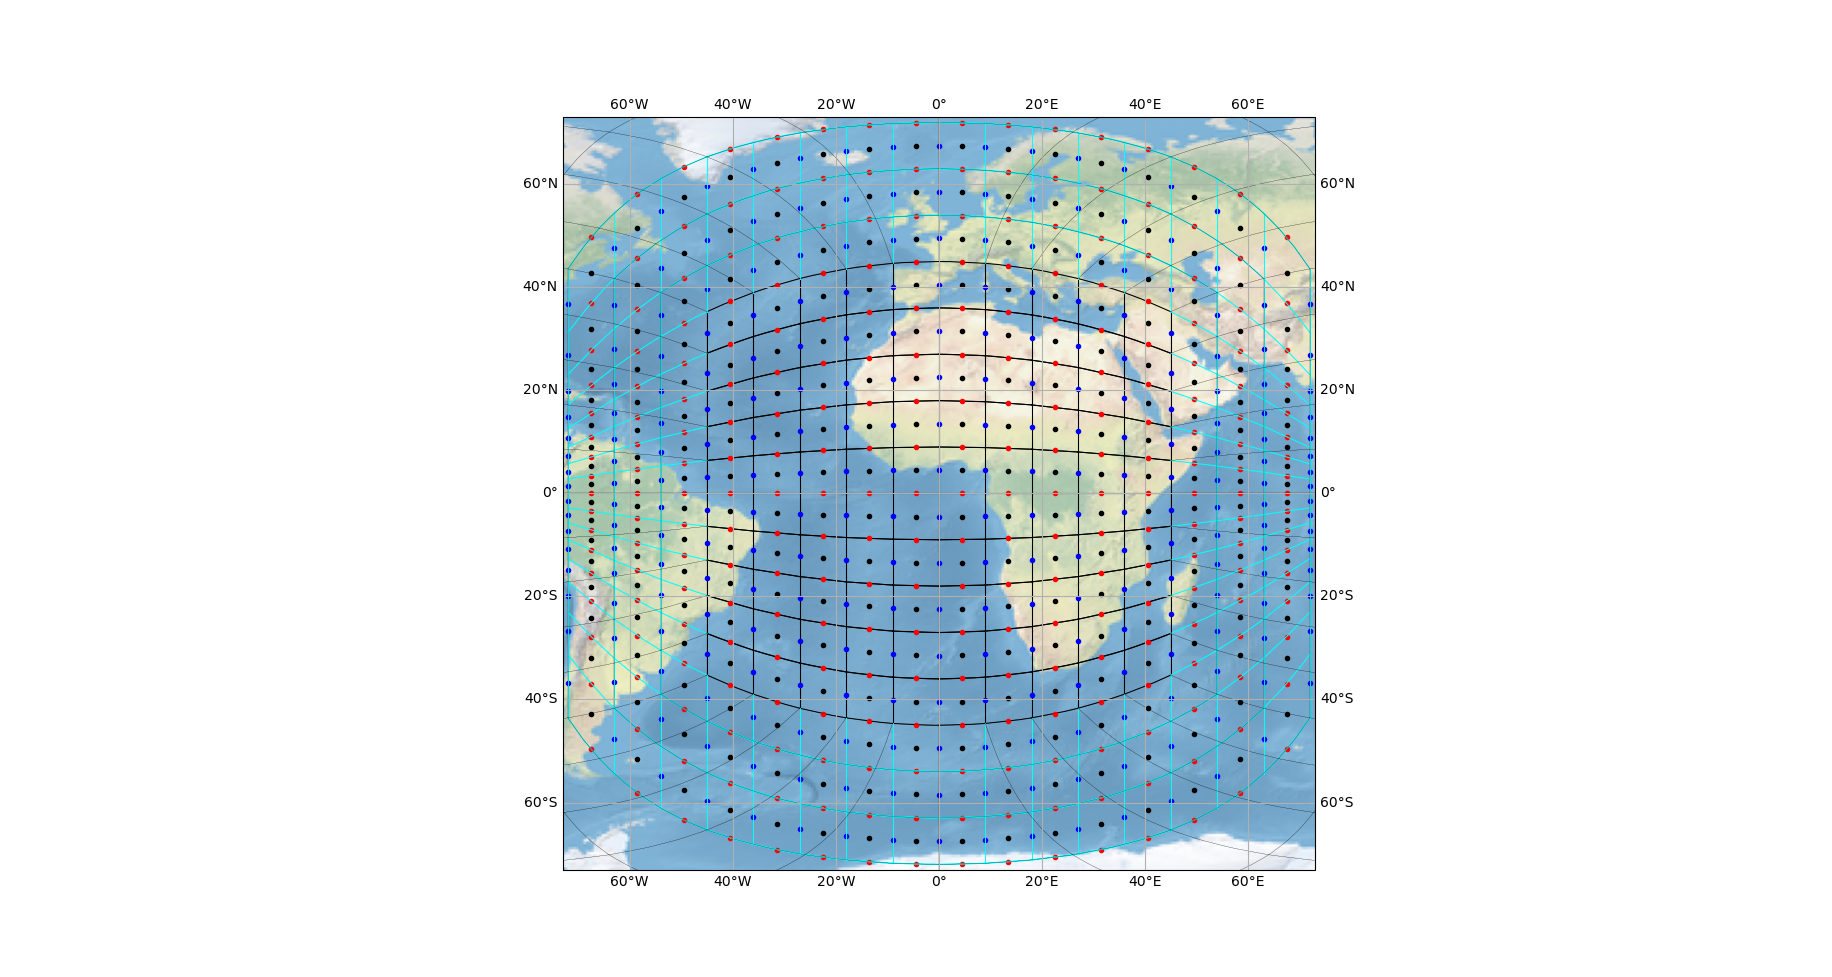
\includegraphics[width=1\linewidth]{gnomonic_equiangular_cs_10_mercator}
	\caption{Grid function at centers (black dots), edge midpoints in the $x$ direction (blue dots)
        and edge midpoints in the $y$ direction (red dots) at panel 1
        for the equiangular cubed-sphere using three layers of ghost cells and $N=10$.
        Ghost cells of panel 1 are drawn using cyan colors.
	\label{chp4-cs-grid-function}}
\end{figure}

We define the average values of a function $q$ with the aid of the metric tensor
$\sigma(x,y)$ at time $t$: 
\begin{equation*}
	Q_{ijp}(t) = \frac{1}{|\Omega_{ijp}|}\int_{x_{i-\frac{1}{2}}}^{x_{i+\frac{1}{2}}}
	\int_{y_{j-\frac{1}{2}}}^{y_{j+\frac{1}{2}}}  q(x,y,p,t) {\sigma(x,y)}\,dx \,dy,
\end{equation*}
where $|\Omega_{ijp}|$ is the control volume area given by:
\begin{equation*}
	|\Omega_{ijp}| = \int_{x_{i-\frac{1}{2}}}^{x_{i+\frac{1}{2}}} \int_{y_{j-\frac{1}{2}}}^{y_{j+\frac{1}{2}}}{\sigma(x,y)} \,dx \,dy.
\end{equation*}
In this context, we define $Q(t) \in \mathcal{CS}_N$ given by 
$Q(t) = (Q_{ijp}(t))_{i,j = -\nu +1, \ldots, N+\nu}^{p=1,\ldots,6}$.
Similar to Proposition \ref{prop-bound-centroid-2d}, we may approximate the average value using the centroid value, that is
\begin{equation*}
	Q_{ijp}^n - q_{ijp}^n = O(\Delta x ^2), 
\end{equation*}
In this work, we shall always approximate the average values since our schemes are expected to be at most second-order,
this approximation does not deteriorate the convergence order.

\section{Edges treatment}
\label{cs-halodata}
\subsection{Ghost cells scalar field interpolation}
\label{cs-interp}
Let's consider a function $q: \mathbb{S}^2_R \to \mathbb{R}$ given at the cell centroids, 
denoted by $q_{ijp}$, where $i, j=1\ldots, N$ and $p=1,\ldots, 6$. 
Our objective is to estimate these values at positions outside the range $1, \ldots, N$, specifically at ghost cell positions.

To solve this problem, we will employ the strategy outlined in \citet{zerroukat:2022}. 
As previously mentioned, the ghost cells in the local Cartesian systems are mapped onto the geodesics 
of adjacent panels, which enables us to use Lagrange interpolation to obtain the values of ghost cells.
\begin{figure}[!htb]
	\centering
	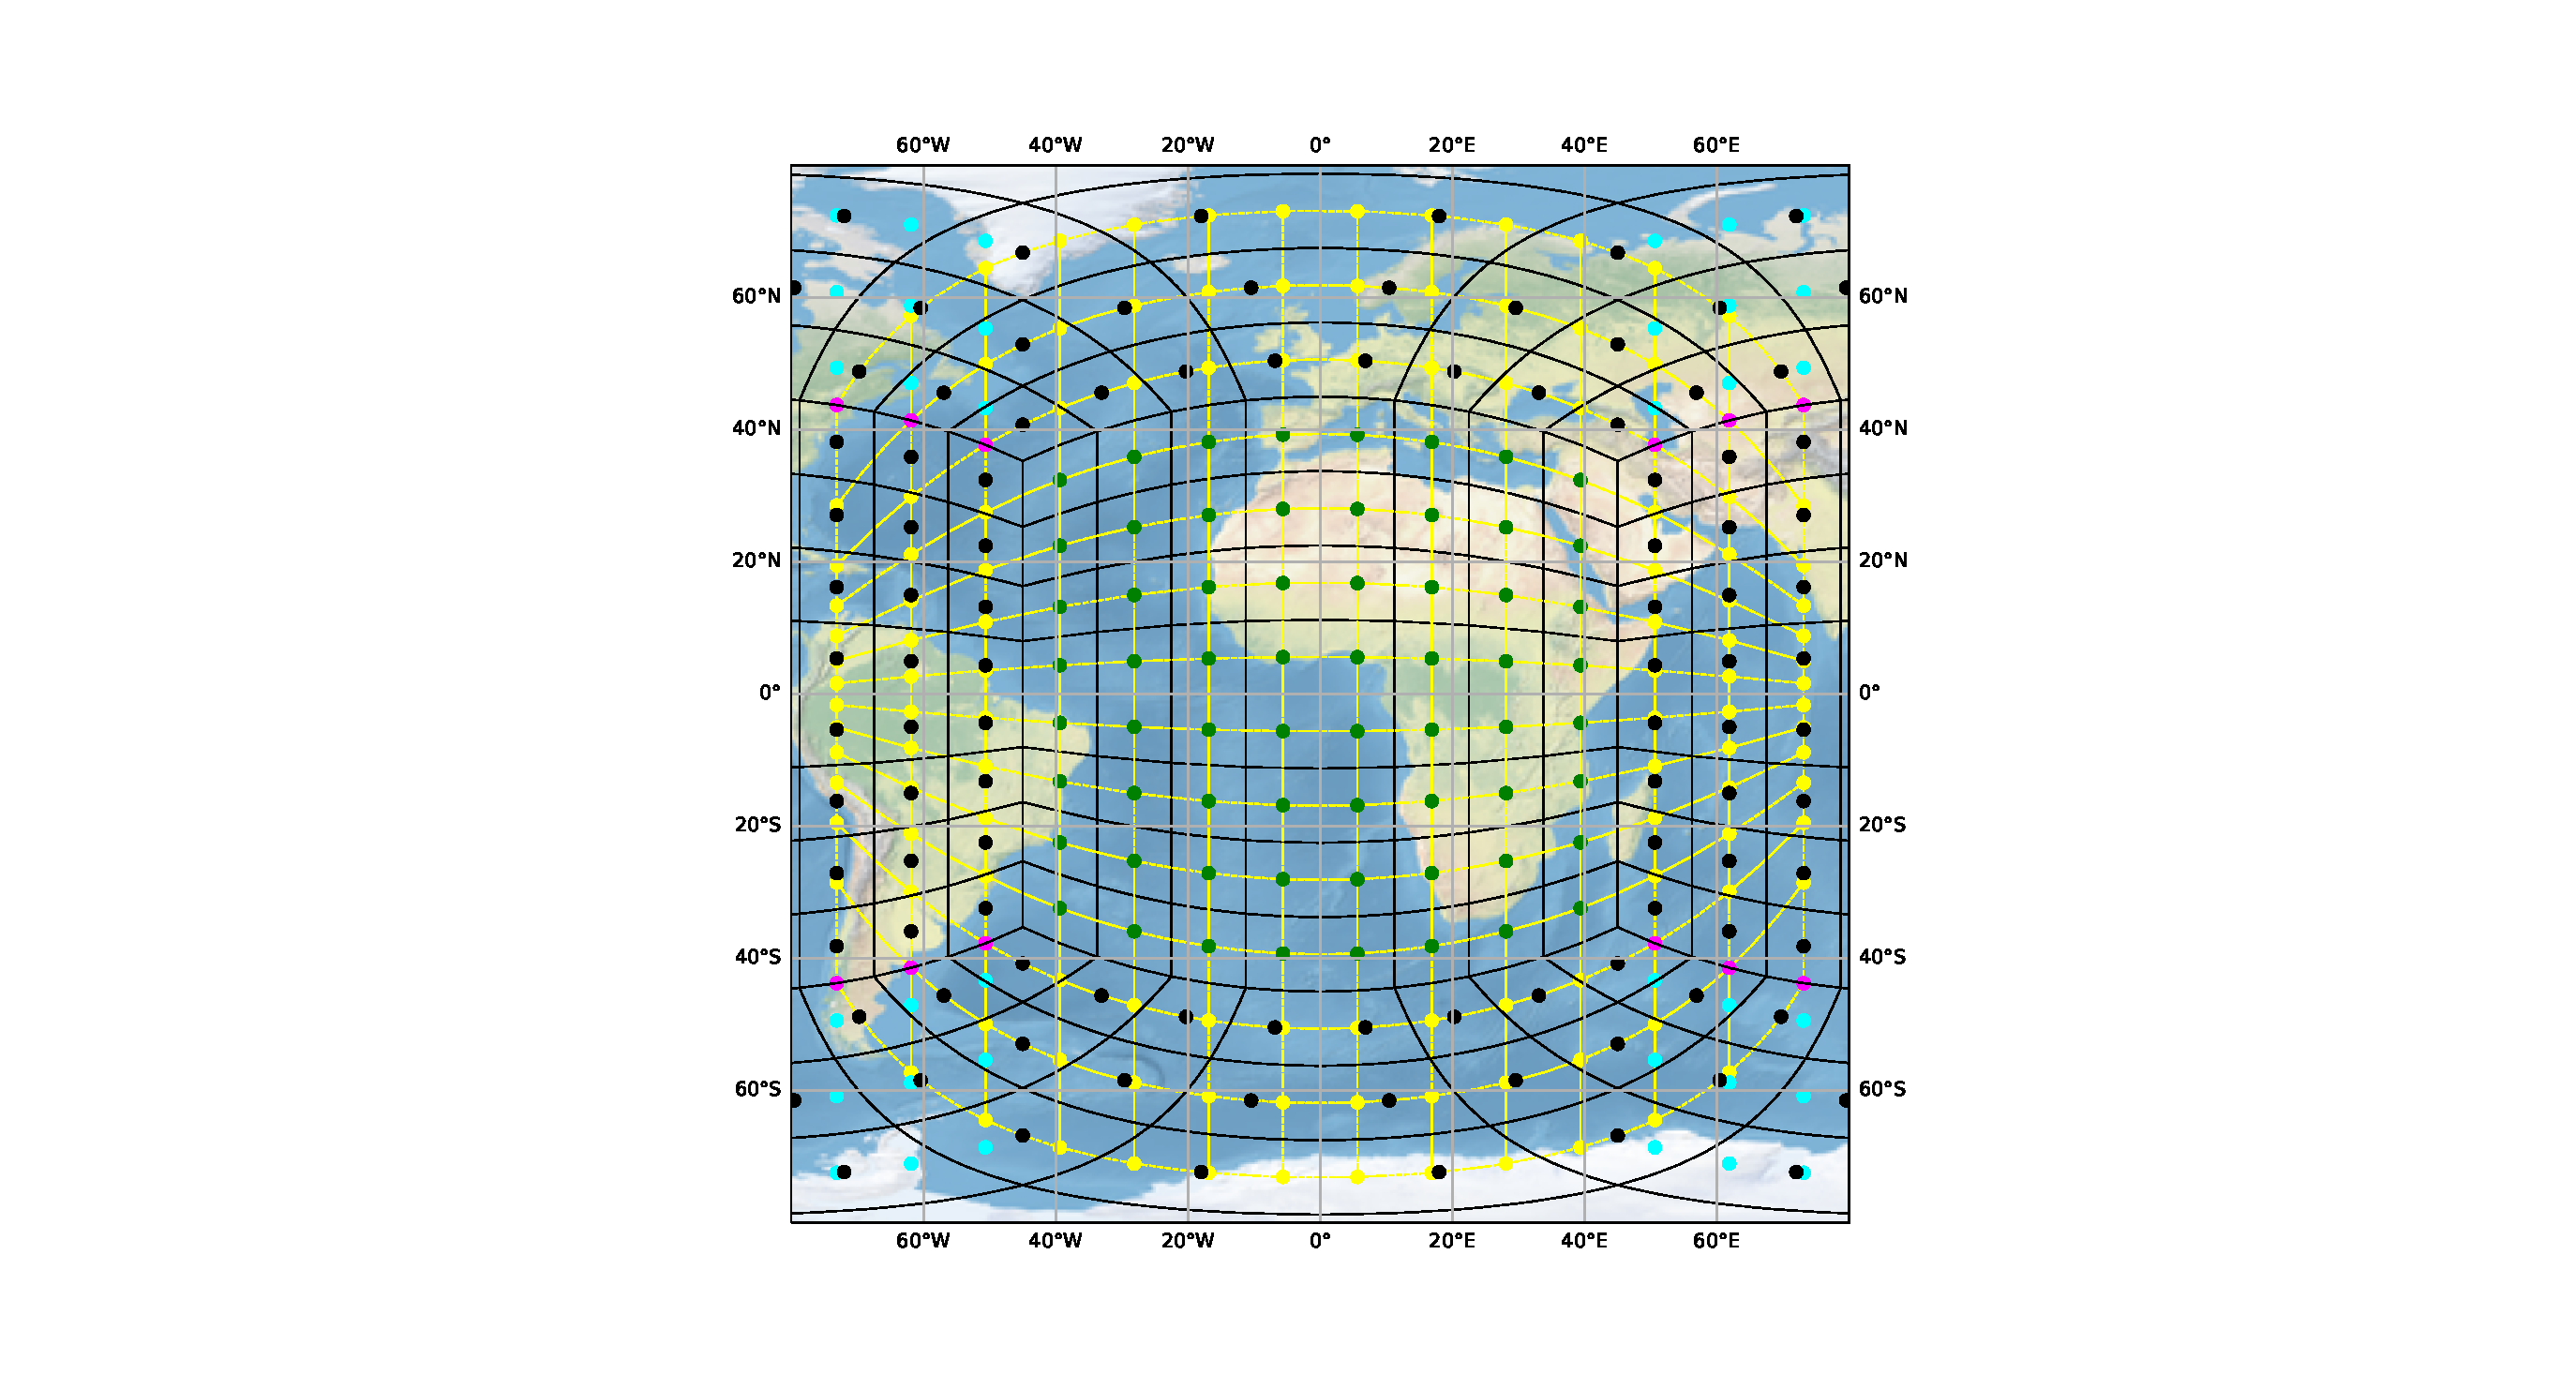
\includegraphics[width=1.0\linewidth]{gnomonic_equiangular_8_mercator}
	\caption{Equiangular cubed-sphere panel 1 with $N=8$: 
	centroid at panel 1 (green circles) and others panel centroids (black circles), 
	ghost cell points at panel 1 (yellow and magenta circles) and others panels (cyan circles).}
	\label{chp4-cs-halodata}
\end{figure}

To illustrate this process in Panel 1, we depict the values of $q_{ijp}$ in Figure \ref{chp4-cs-halodata}. 
The green circles represent the values in Panel 1, while the black circles 
represent the values in the other panels, for a given $N=8$. 
Assuming a halo size of 3, we also indicate the target values at the ghost cell 
positions using yellow and magenta circles. 
It is worth noting that the dashed yellow lines in Figure \ref{chp4-cs-halodata} 
illustrate how the ghost cell points lie on geodesics containing grid positions from adjacent panels.
With the exception of the magenta circles, all the ghost cell values can be obtained using 1D Lagrange interpolation, 
utilizing the surrounding black circles on the geodesic. 
This interpolation procedure can be performed for all panels. 
Subsequently, the magenta circles can be interpolated using the values obtained in the first step of interpolation 
(depicted as cyan circles in Figure \ref{chp4-cs-halodata}), 
while preserving the order of accuracy of the interpolation, assuming it is fixed. 
\begin{figure}[!htb]
	\centering
	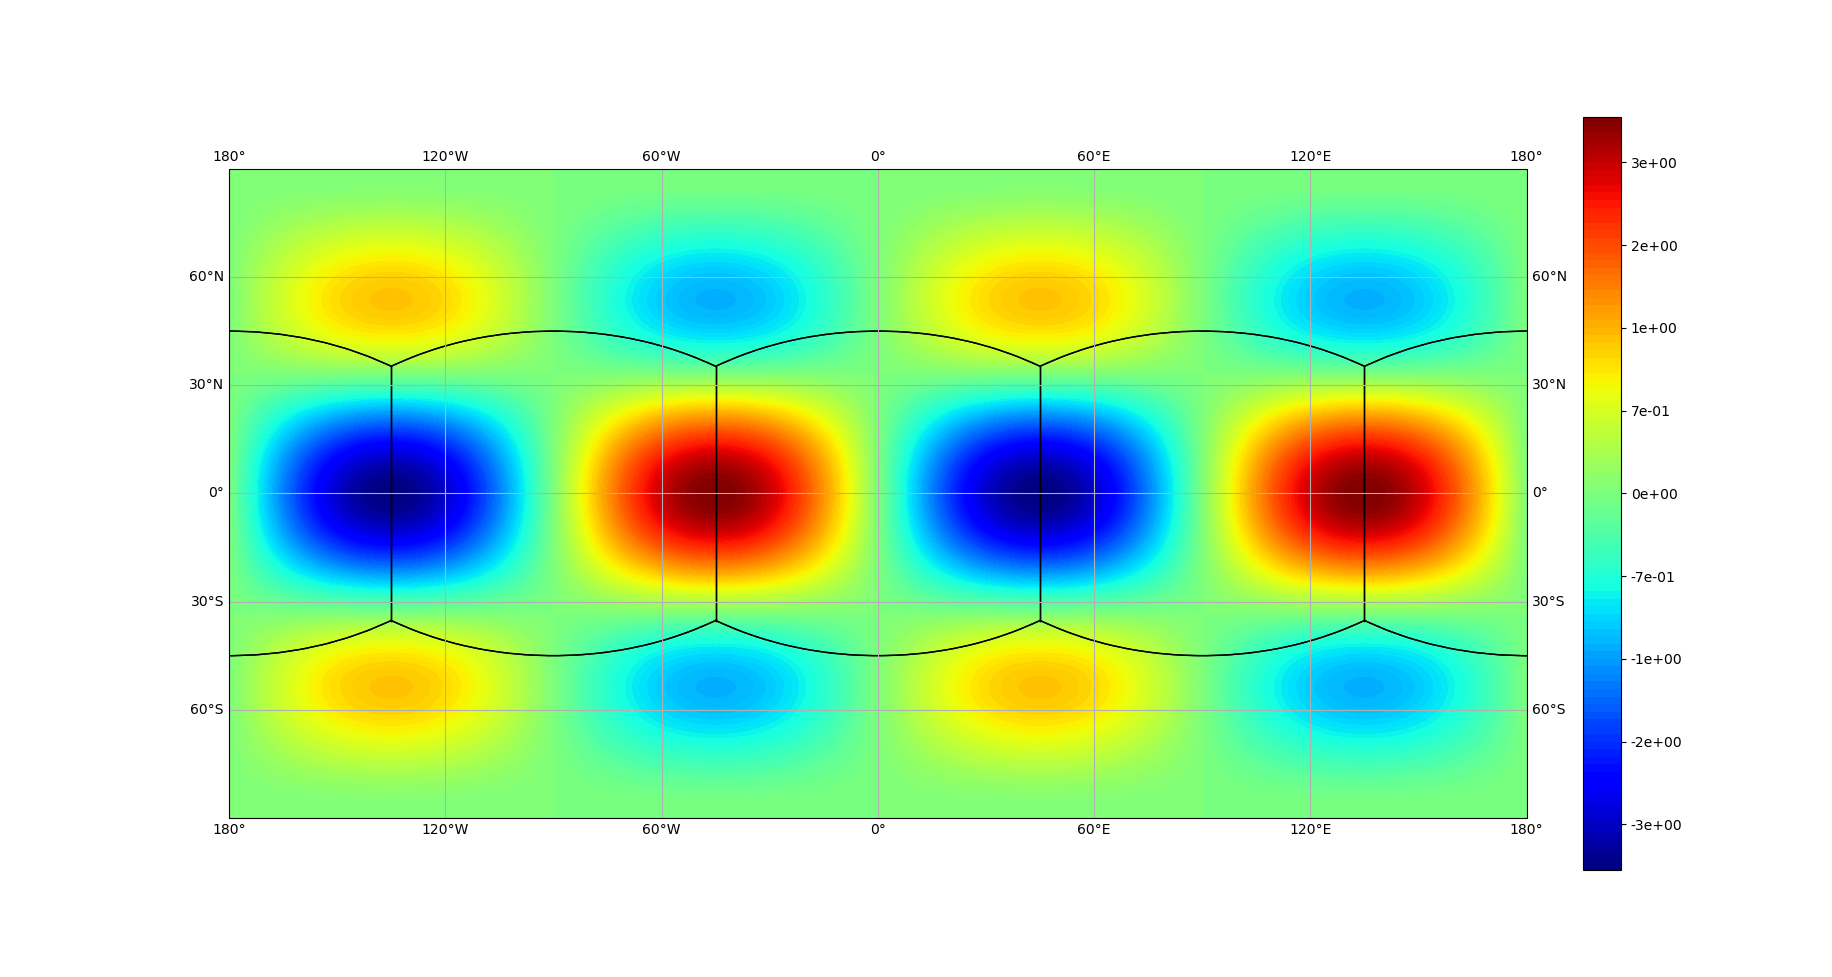
\includegraphics[width=0.8\linewidth]{gnomonic_equidistant_1024_interp_q_ic_2_mercator}
	\caption{Trigonometric function defined by Equation \eqref{chp4-ic2}.}
	\label{chp4-cs-ic2}
\end{figure}

We are going to show a numerical example of this interpolation process using a halo region of size 4 and 
assuming the radius of the sphere is equal to one.
We shall consider the following trigonometric function, which is the divergence of a velocity field,
as in \citet{peixoto:13} in our tests:
\begin{align}
	\label{chp4-ic2}
	\begin{split}
	q(\lambda, \phi) = \frac{1}{\cos(\phi)}\bigg(-2\cos^3(\phi) \sin(\lambda) \cos(\lambda)
	+16\sin^2(\lambda)\cos(\lambda)\cos^3(\phi)\sin(\phi)\bigg),
	\end{split}
\end{align}
whose graph is depicted in Figure \ref{chp4-cs-ic2}.
\begin{figure}[!htb]
	\centering
	\begin{subfigure}{0.45\textwidth}
		\centering
		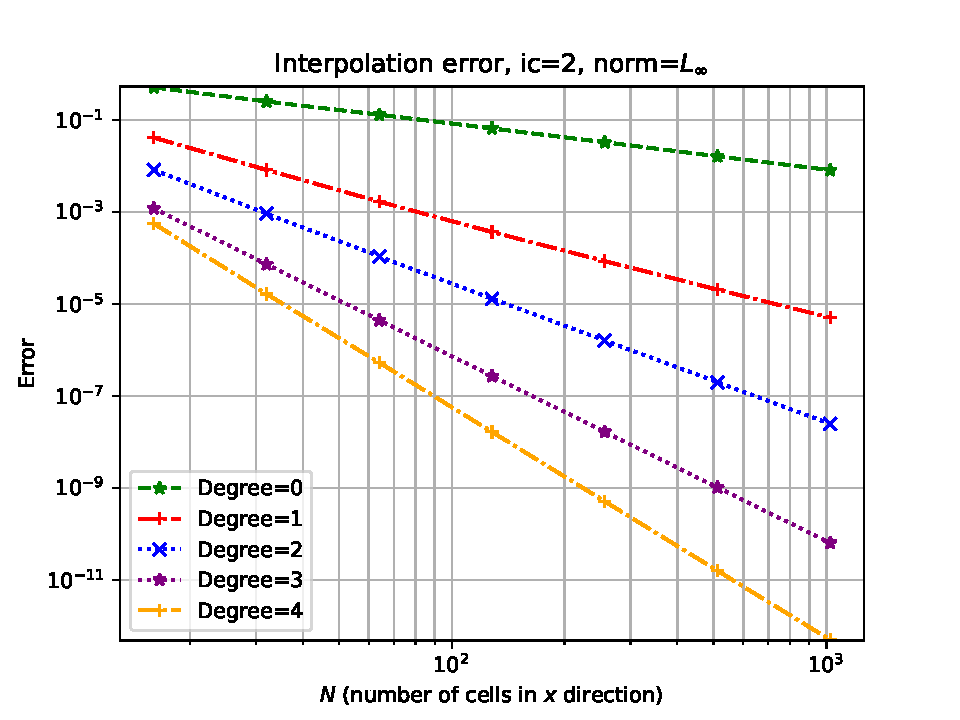
\includegraphics[width=1\linewidth]{cs_interp_ic2_normlinf_errors}
		\caption{Error.\label{chp4-exp2-error}}
	\end{subfigure}
	\begin{subfigure}{0.45\textwidth}
		\centering
		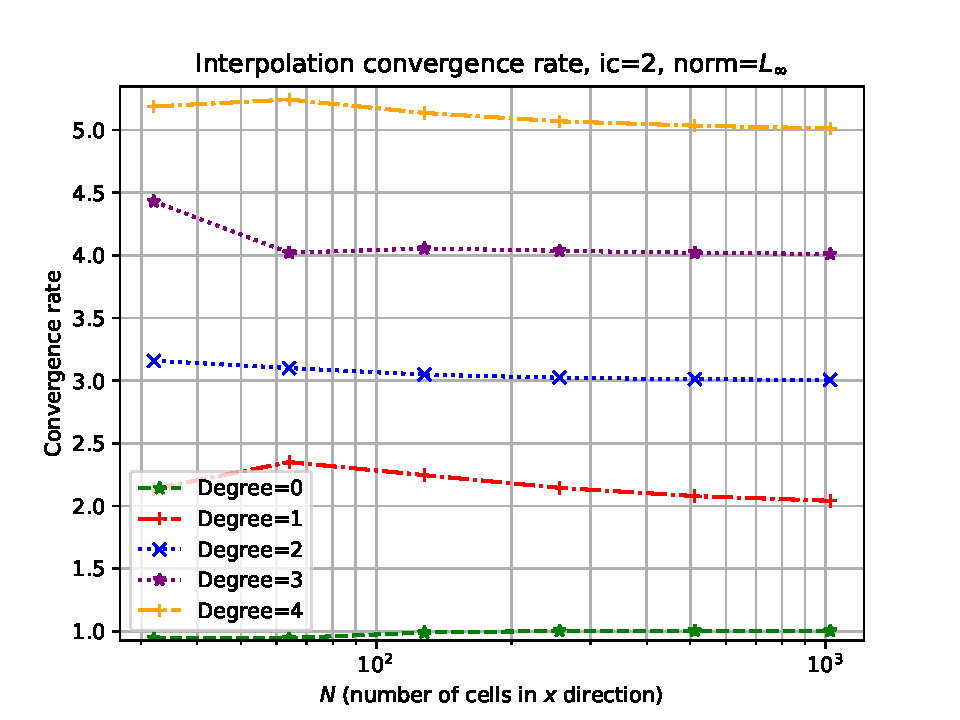
\includegraphics[width=1\linewidth]{cs_interp_ic2_normlinf_convergence_rate}
		\caption{Convergence rate.\label{chp4-exp2-CR}}
	\end{subfigure}
	\caption{Relative error convergence (a) and convergence rate (b) for the ghost cell interpolation process for different
		polynomial degrees, using the trigonometric function given by Equation \eqref{chp4-ic2}.\label{chp4-exp2}}
\end{figure}

We are going to consider the relative error in the maximum norm and the convergence rate 
at the ghost cell positions defined analogously as in Section \ref{sec-ds-exp}. 
We also consider values os $N$ given by $2^k$, for $k=4, \ldots, 10$, in order to compute the error and convergence rate.
In Figures \ref{chp4-exp2} we show the error and convergence rate for the trigonometric function (Equation \eqref{chp4-ic2}),
respectively, considering polynomials of degrees from 0 up to 4. As both graphs show, we were able to achieve the expected order of convergence.

\subsection{Ghost cells wind interpolation}
\label{cs-wind-interp}
Let us consider the following problem: Assume that we are given a tangent vector field of the sphere, denoted as 
$\boldsymbol{u}:\mathbb{S}^2_R \to \mathbb{R}^3$. We also have its contravariant components at the control-volume
midpoints, namely $u_{i+\frac{1}{2},j,p}$ for $i=0, \ldots, N$ and $j=1, \ldots, N$, as well as
$v_{i,j+\frac{1}{2},p}$ for $i=1, \ldots, N$ and $j=0, \ldots, N$.

Our objective is to obtain the values 
\begin{align*}
u_{i+\frac{1}{2},j,p} \quad \text{ for} \quad &i=-1, \ldots, N+1, \quad &j=-\nu+1, \ldots, 0, \quad &j=N, \ldots, N+\nu,\\
v_{i,j+\frac{1}{2},p} \quad \text{ for} \quad &j=0, \ldots, N, \quad &i=-\nu+1, \ldots, 0,\quad &i=N, \ldots, N+\nu,
\end{align*}
as shown in Figure \ref{chp4-wind-interp}. This problem arises when we apply the dimension splitting method on each panel of the cubed-sphere.
\begin{figure}[!htb]
	\centering
	\begin{subfigure}{1\textwidth}
		\centering
		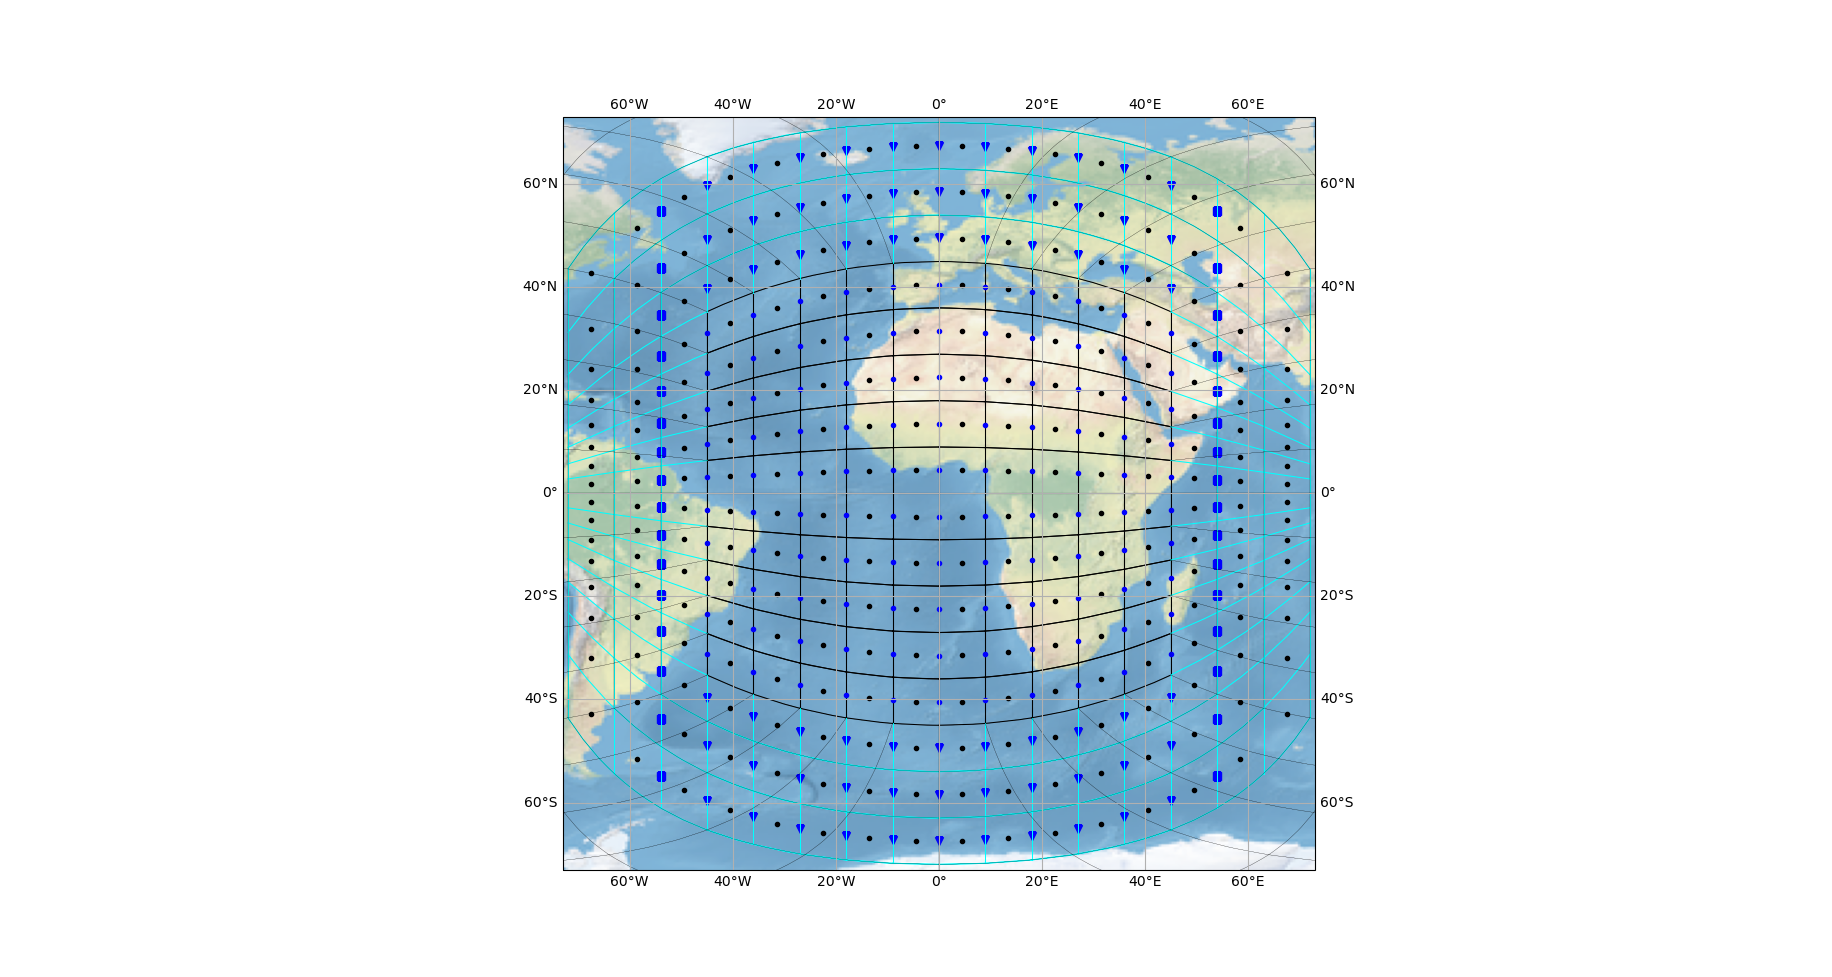
\includegraphics[width=1\linewidth]{gnomonic_equiangular_cs_10_mercator_x}
		\caption{Contravariant component $u$. \label{chp4-wind-interp-a}}
	\end{subfigure}
	\begin{subfigure}{1\textwidth}
		\centering
		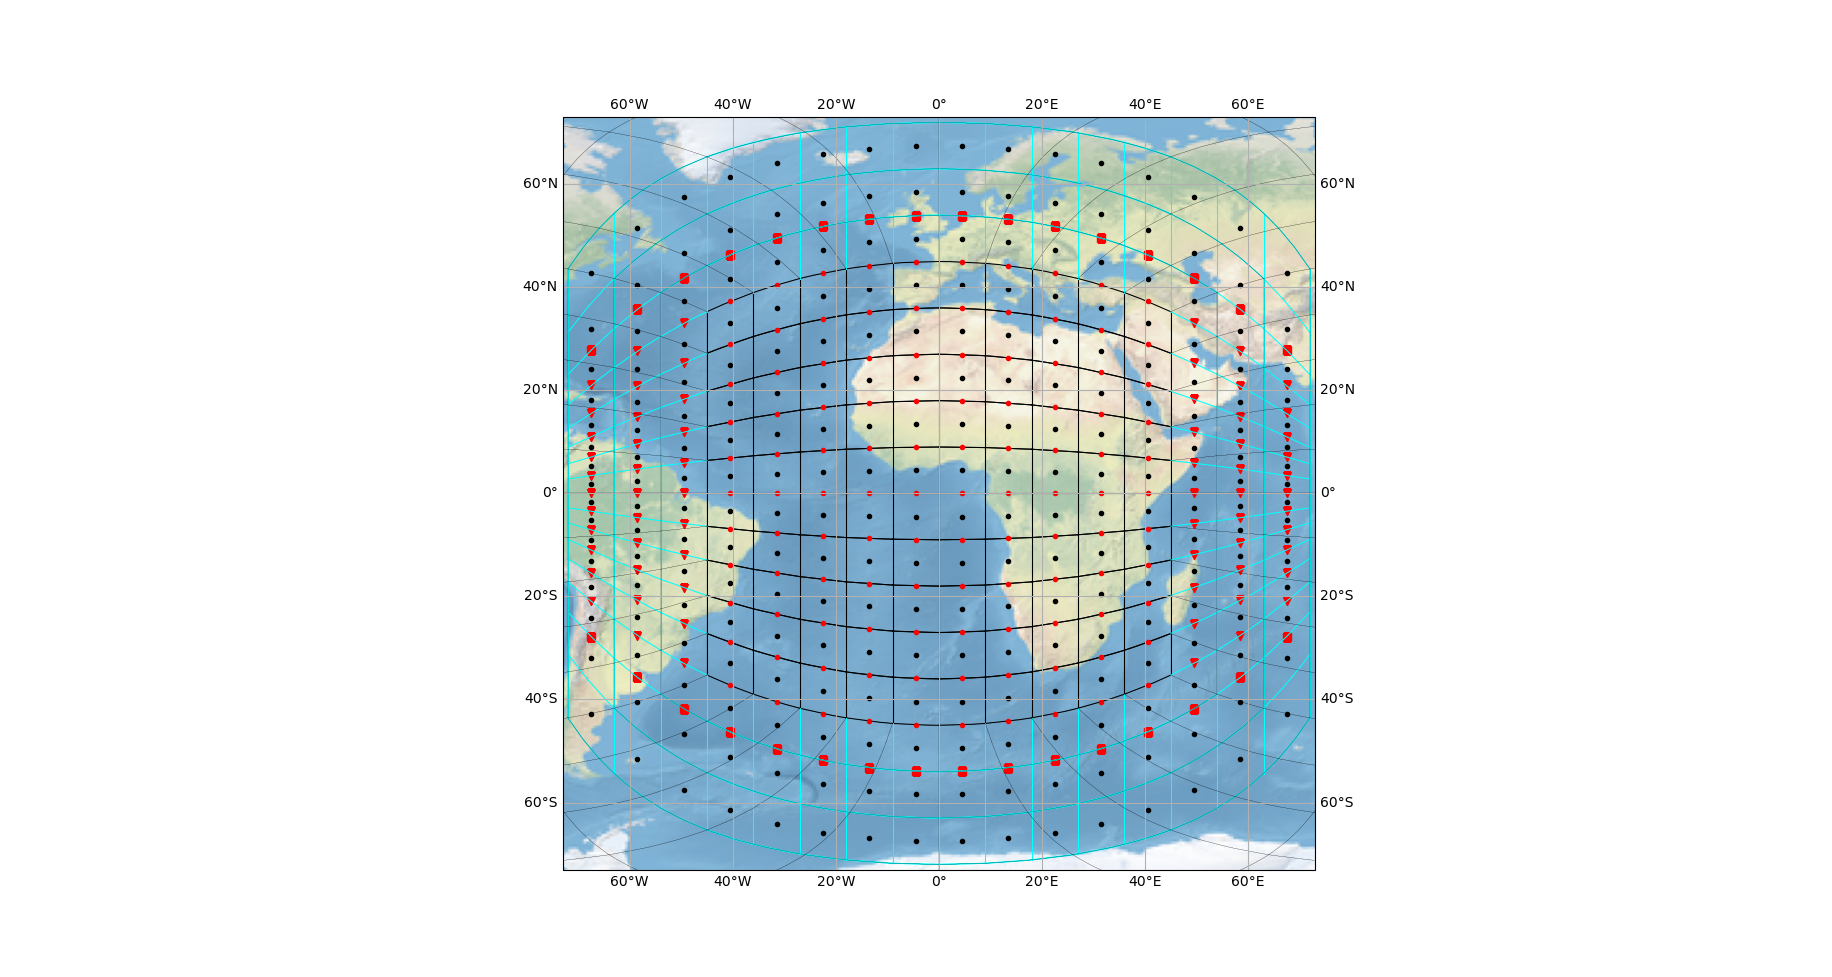
\includegraphics[width=1\linewidth]{gnomonic_equiangular_cs_10_mercator_y}
		\caption{Contravariant component $v$. \label{chp4-wind-interp-b}}
	\end{subfigure}
	\caption{ Illustration of contravariant components $u$ (a) and $v$ (b) of a vector field at edge midpoints.
		Ghost cell points are denoted by triangles and squares.
		The extra points needed for the RK2 scheme are denoted by squares.\label{chp4-wind-interp}}
\end{figure}


This problem can be solved by using the interpolation process described earlier for a scalar field.
To apply the interpolation process, we first need to interpolate the values of $u$ and $v$ from the
edges to the centers at the points required for the ghost cells interpolation. Specifically, we need the values:
\begin{align*}
	u_{1+k,j,p}, v_{1+k,j,p} \quad \text{ for} \quad &j=1, \ldots, N, \quad k=0, \ldots, \nu-1,\\
	u_{N-k,j,p}, v_{N-k,j,p} \quad \text{ for} \quad &j=1, \ldots, N, \quad k=0, \ldots, \nu-1,\\
	u_{i,1+k,p}, v_{i,1+k,p} \quad \text{ for} \quad &i=1, \ldots, N, \quad k=0, \ldots, \nu-1,\\
    u_{i,N-k,p}, v_{i,N-k,p} \quad \text{ for} \quad &i=1, \ldots, N, \quad k=0, \ldots, \nu-1.\\
\end{align*}
We apply a third-order interpolation in the $x$ direction of each panel to interpolate $u$ from the edges to the centers
(see Figure \ref{chp4-wind-interp-a}). Similarly, we use a third-order interpolation to obtain the values of $v$ at the 
centers in the $y$ direction (see Figure \ref{chp4-wind-interp-b}).
Once these interpolated values are computed, we convert the contravariant values $u_{ijp}, v_{ijp}$
to their latitude-longitude components $(u_{\lambda})_{ijp}, (v_{\phi})_{ijp}$ using Equation
\eqref{contravariant-to-ll}. This conversion avoid any coordinate system discontinuity.
Then, we can use the ghost cell centers interpolation procedure described before for the latitude-longitude components
to recover the wind at the ghost cell centers using any polynomial degree.
Finally, we can use the values at the ghost cell centers to obtain the values at the ghost cell edges
by employing a third-order interpolation once again.
Subsequently, the contravariant components can be obtained by using Equation \eqref{ll-to-contravariant}.

We will consider the following rotated zonal field on the unit sphere, as a numerical test, based on \citet{will:1992}:
\begin{align}
	\label{chp4-wind1}
	\begin{cases}
		u_\lambda(\lambda,\phi,t) = u_0(\cos(\phi)\cos(\alpha) + \sin(\phi)\cos(\lambda)\sin(\alpha)),\\
		v_\phi(\lambda,\phi,t) = -u_0\sin(\lambda)\sin(\alpha).
	\end{cases}
\end{align}
Here, $u_0=\frac{2\pi}{5}$ and $\alpha= -\frac{45\pi}{180}$. We will adopt the same grids as in Section \ref{cs-interp}.
Next, we will compute the relative errors of the contravariant components at the midpoint edges,
as depicted in Figure \ref{chp4-wind-interp-a} and Figure \ref{chp4-wind-interp-b}.
The errors are presented in Figure \ref{chp4-expvf}, along with the convergence rate for different degrees employed in the ghost cell center interpolation.
We emphasize that, since we utilize a third-order interpolation to retrieve the wind at centers from the edges, as well as in the interpolation
from the ghost cell centers to ghost cell edges, the maximum attainable scheme order is 4.
Indeed, from Figure \ref{chp4-expvf}, we observe that when employing a fourth-order interpolation in the ghost cell interpolation step, the final order achieved is 4.
\begin{figure}[!htb]
	\centering
	\begin{subfigure}{0.45\textwidth}
		\centering
		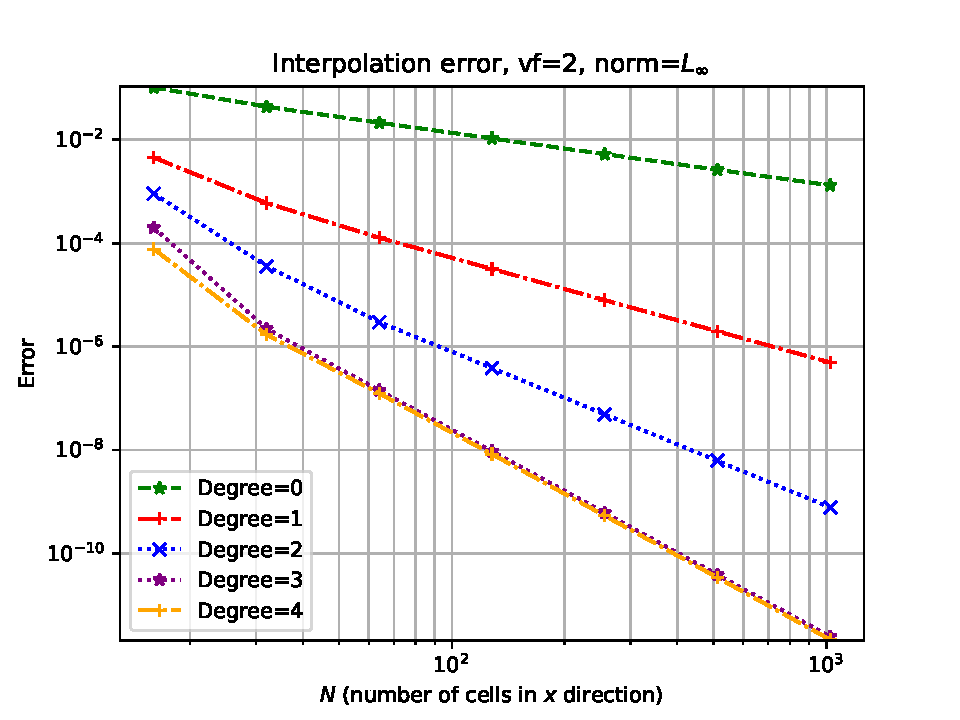
\includegraphics[width=1\linewidth]{cs_interp_vf2_normlinf_errors}
		\caption{Error.\label{chp4-exp-vf-error}}
	\end{subfigure}
	\begin{subfigure}{0.45\textwidth}
		\centering
		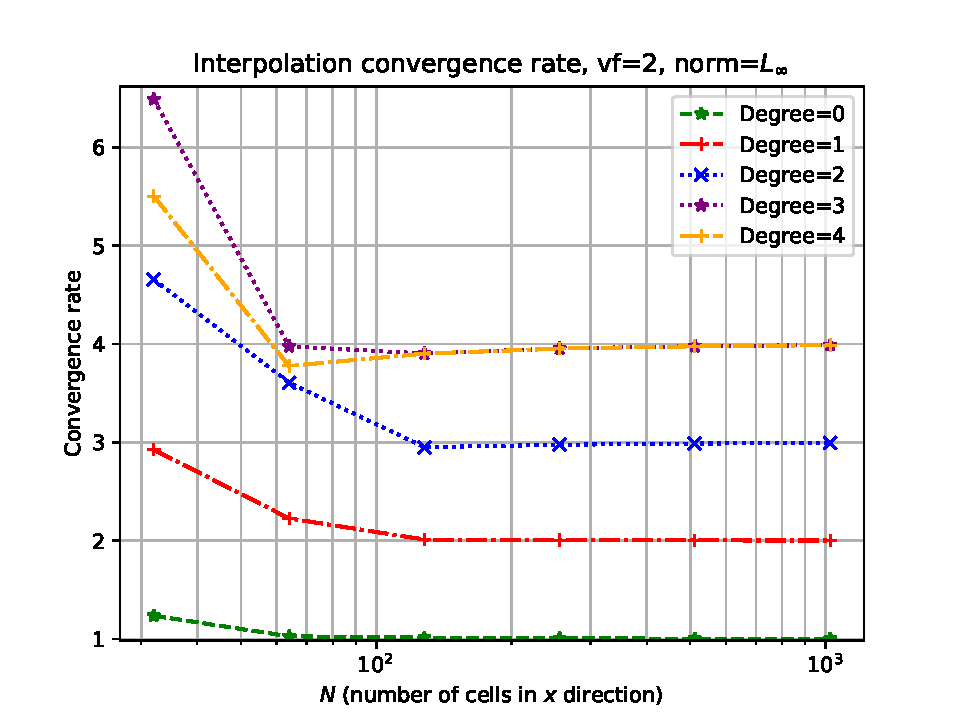
\includegraphics[width=1\linewidth]{cs_interp_vf2_normlinf_convergence_rate}
		\caption{Convergence rate.\label{chp4-exp-vf-CR}}
	\end{subfigure}
	\caption{Relative error convergence (a) and convergence rate (b) for the ghost cell interpolation of a vector field process for different
	polynomial degrees, using the trigonometric function given by Equation \eqref{chp4-wind1}.\label{chp4-expvf}}
\end{figure}
\subsection{Edges reconstruction}
\label{cs-recon}
Let us consider the following problem: given the values $q_{ijp}$ we wish to find 
approximations of the function $q$ at the control volume edge midpoints denoted by
\begin{align*}
q^{L,x}_{ijp}  \approx q_{{i-\frac{1}{2}},j,p},\quad
q^{R,x}_{ijp}  \approx q_{{i+\frac{1}{2}},j,p},\quad
q^{L,y}_{ijp}  \approx q_{i,{j-\frac{1}{2}},p},\quad
q^{R,y}_{ijp}  \approx q_{i,{j+\frac{1}{2}},p}.
\end{align*}
These points are illustrated in Figure \ref{csgrid-rpoints} for panel 1.
\begin{figure}[!htb]
	\centering
	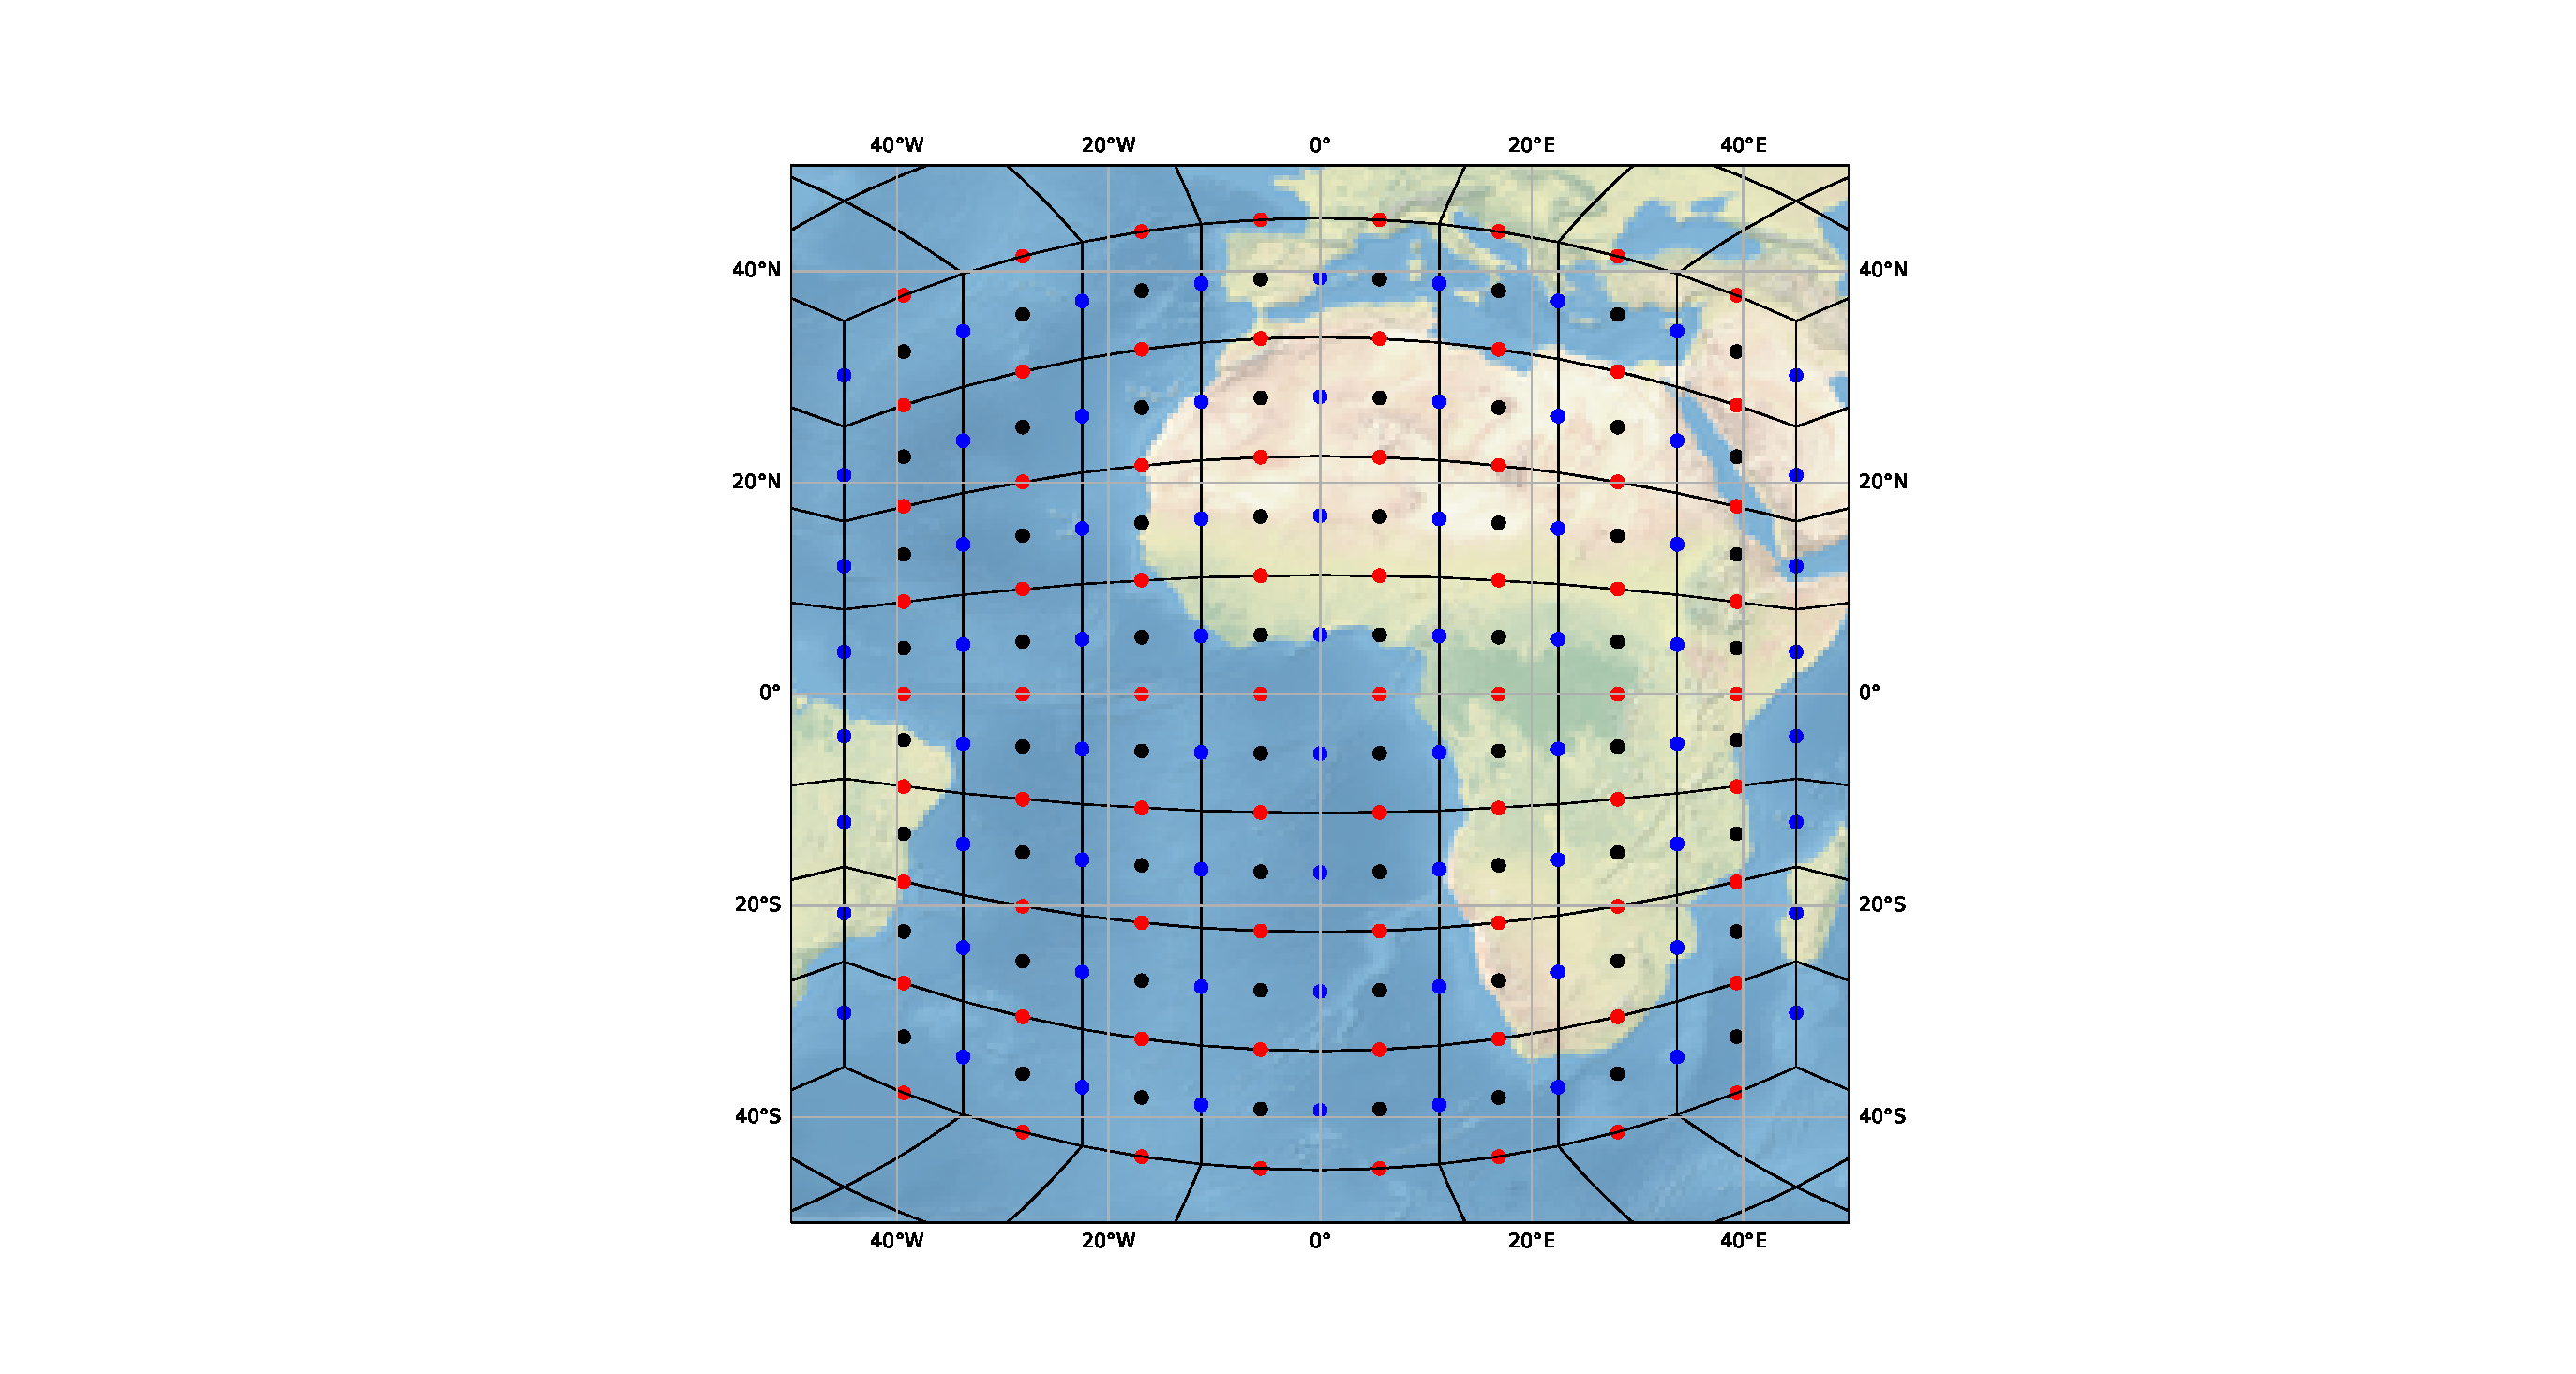
\includegraphics[width=1\linewidth]{gnomonic_equiangular_8_mercator_2}
	\caption{The reconstruction problem on the cubed-sphere panel 1: we are given the centroid values of a function (black circles)
		and we wish to estimate these values at the edges midpoints in the $x$ direction (blue circles) and $y$ direction (red circles).
		This figure uses an equiangular cubed-sphere with $N=8$.} \label{csgrid-rpoints}
\end{figure}

We can estimate the desired values by using the one-dimensional reconstruction schemes 
described in Sections \ref{chp2-sec-recon} and \ref{chp2-sec-mono}, 
performing PPM reconstruction independently in the $x$ and $y$ directions. 
It is worth noting that all the schemes discussed in those sections are 
expected to be second-order accurate due to the centroid point approximation.

However, there are differences in the computation of the stencil near the cube edges. 
Unlike in the previous chapters, where periodic boundary conditions were assumed, 
the boundary conditions in this context are related to the adjacent panels. 
One way to address this issue is by adding ghost cell layers and utilizing 
the process described in Section \ref{cs-interp} to compute the stencils. 
This approach is referred to as \textbf{ET-ZA22} (Edge Treatment - ZA22), 
as it extends the grid lines and employs Lagrange interpolation, 
as described by \citet{zerroukat:2022}.
\begin{figure}[!htb]
	\centering
	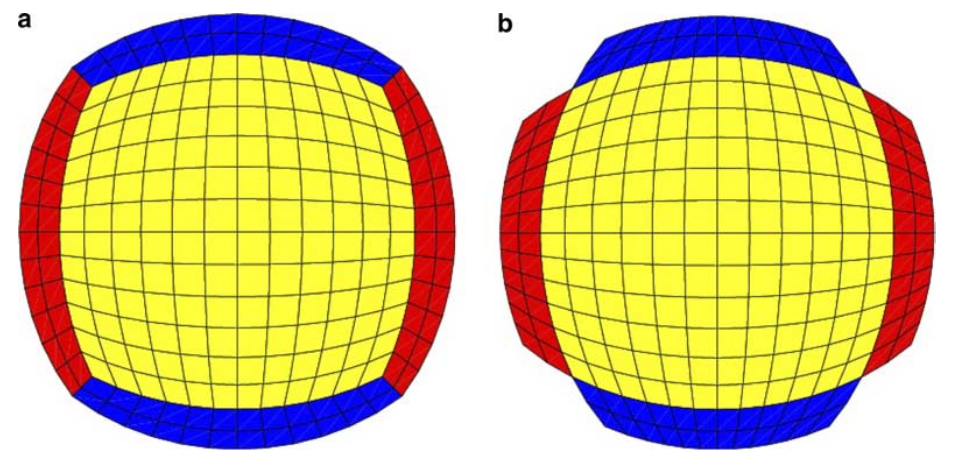
\includegraphics[width=0.8\linewidth]{haloregion}
	\caption{Different approaches for defining the halo region:
    (a) using adjacent cell values (used in ET-S72 and ET-PL07);
    (b) extending the panel grid lines (used in ET-ZA22). 
    Figure taken from \citet{ross:2006} \label{chp4-haloregion}}
\end{figure}

Another approach, employed in \citet{sadourny:1972}, involves ignoring the
discontinuity of the coordinate system and simply using the values of the cells 
in the adjacent panels as the ghost cell values. This scheme is labeled \textbf{ET-S72} (Edge Treatment - S72).

Additionally, an alternative method that avoids the use of ghost cells was developed by
\citet{putman:2007}, which entails extrapolation at the cells surrounding the cube edge.
We will refer to this scheme as \textbf{ET-PL07} (Edge Treatment - PL07).
This scheme uses the following extrapolations:
\begin{align*}
	q^{L,x}_{1,j,p} &= \frac{1}{2}\bigg(3Q_{1,j,p} - Q_{2,j,p}\bigg),\\
	q^{R,x}_{N,j,p} &= \frac{1}{2}\bigg(3Q_{N,j,p} - Q_{N-1,j,p}\bigg),\\
	q^{L,y}_{i,1,p} &= \frac{1}{2}\bigg(3Q_{i,1,p} - Q_{i,2,p}\bigg),\\
	q^{R,y}_{i,N,p} &= \frac{1}{2}\bigg(3Q_{i,N,p} - Q_{i,N-1,p}\bigg),\\
\end{align*}
at the points that are located on the cube edges. The other edge values are estimated as:
\begin{align*}
	q^{R,x}_{1,j,p} &= \frac{1}{14}\bigg(3Q_{1,j,p} + 11Q_{2,j,p} - 2(Q_{3,j,p} - Q_{1,j,p})\bigg),\\
	q^{L,x}_{2,j,p} &= q^{R,x}_{1,j,p},\\
	q^{L,x}_{N,j,p} &= \frac{1}{14}\bigg(3Q_{N,j,p} + 11Q_{N-1,j,p} - 2(Q_{N-2,j,p} - Q_{N,j,p})\bigg),\\
	q^{R,x}_{N-1,j,p} &= q^{L,x}_{N,j,p},\\
\end{align*}
in the $x$ direction and in the $y$ direction we use the formulas
\begin{align*}
	q^{R,y}_{i,1,p} &= \frac{1}{14}\bigg(3Q_{i,1,p} + 11Q_{i,2,p} - 2(Q_{i,3,p} - Q_{i,1,p})\bigg),\\
	q^{L,y}_{i,2,p} &= q^{R,x}_{i,1,p},\\
	q^{L,y}_{i,N,p} &= \frac{1}{14}\bigg(3Q_{i,N,p} + 11Q_{i,N-1,p} - 2(Q_{i,N-2,p} - Q_{i,N,p})\bigg),\\
	q^{R,y}_{i,N-1,p} &= q^{L,y}_{i,N,p}.\\
\end{align*}
We are going to use the trigonometric function (Equation \eqref{chp4-ic2})
as before on the unit sphere to compare the schemes ET-ZA22, ET-S72 and ET-PL07. The scheme ET-ZA22 uses cubic polynomials.
We introduce the relative errors:
\begin{align*}
	e_{{i-\frac{1}{2}},j,p} &= (|q_{{i-\frac{1}{2}},j,p} - q^{L,x}_{ijp}|)/|q_{{i-\frac{1}{2}},j,p}|,\\
	e_{{i+\frac{1}{2}},j,p} &= (|q_{{i+\frac{1}{2}},j,p} - q^{R,x}_{ijp}|)/|q_{{i+\frac{1}{2}},j,p}|,\\
	e_{i,{j-\frac{1}{2}},p} &= (|q_{i,{j-\frac{1}{2}},p} - q^{L,y}_{ijp}|)/|q_{i,{j-\frac{1}{2}},p}|,\\
	e_{i,{j+\frac{1}{2}},p} &= (|q_{i,{j+\frac{1}{2}},p} - q^{R,y}_{ijp}|)/|q_{i,{j+\frac{1}{2}},p}|,\\
	e_{ijp} &= \max\{e_{{i-\frac{1}{2}},j,p}, e_{{i+\frac{1}{2}},j,p} , e_{i,{j-\frac{1}{2}},p}, e_{i,{j+\frac{1}{2}},p} \},\\
	E &= \max \{e_{ijp}\}.
\end{align*}
We are going to compute $E$ for different values of $N$ as in the numerical experiments of Section \ref{cs-interp}.
\begin{figure}[!htb]
	\centering
	\begin{subfigure}{0.45\textwidth}
		\centering
		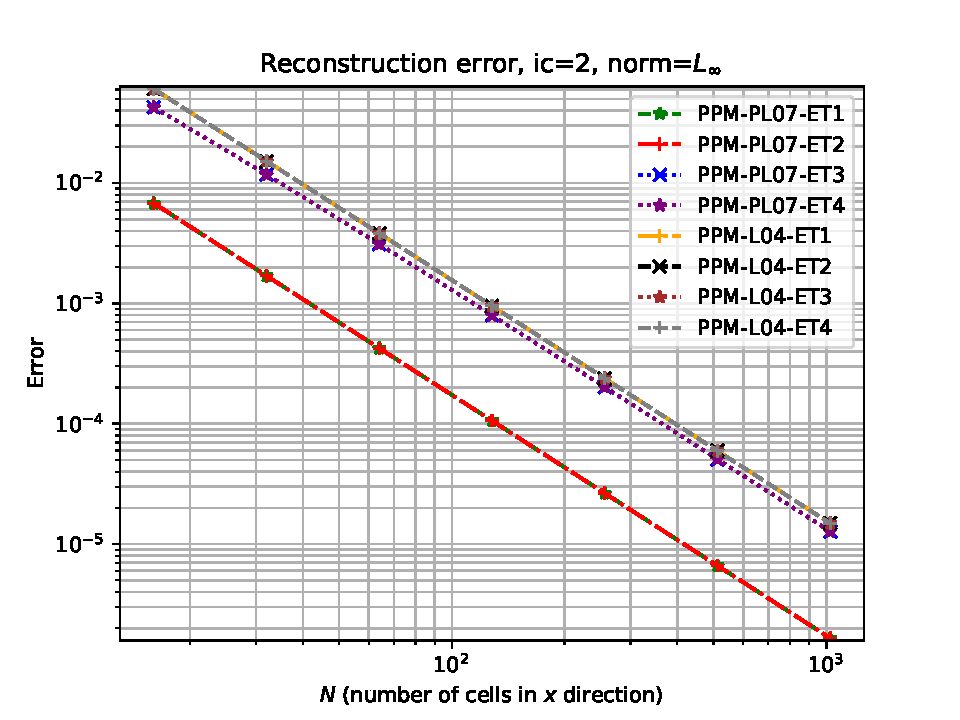
\includegraphics[width=1\linewidth]{cs_recon_ic2_normlinf_parabola_errors}
		\caption{Error.\label{chp4-exp3-error}}
	\end{subfigure}
	\begin{subfigure}{0.45\textwidth}
		\centering
		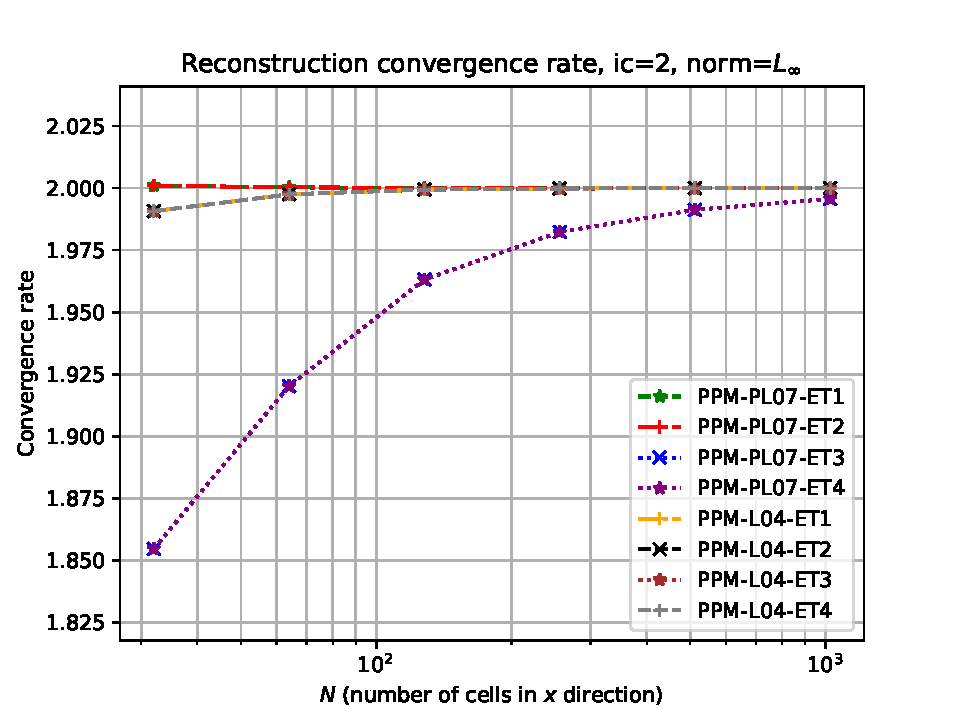
\includegraphics[width=1\linewidth]{cs_recon_ic2_normlinf_convergence_rate}
		\caption{Convergence rate.\label{chp4-exp3-CR}}
	\end{subfigure}
	\caption{Relative error convergence (a) and convergence rate (b) for the reconstruction problem for different
	edge treatments (ET), using the trigonometric function given by Equation \eqref{chp4-ic2}.\label{chp4-exp3}}
\end{figure}

In Figure \ref{chp4-exp3} we show the errors and the convergence rate using the PPM-PL07 and PPM-L04 reconstruction schemes.
We can observe that all the schemes converge to zero with second-order.
The difference between the edge treatments ET-S72, ET-PL07 and ET-ZA22 schemes
may be observed in Figure \ref{chp4-exp4} and Figure \ref{chp4-exp5}, for the  PPM-PL07 and PPM-L04 reconstruction schemes, respectively.
We notice that the cube edges appear on the error graph when we use the ET-S72 and ET-PL07 schemes. This is an example of grid imprinting.
Although all schemes are second-order, the scheme ET-ZA22 do not seem to produce grid imprinting in the reconstruction problem.
\begin{figure}[!ht]
	\centering
	\begin{subfigure}{0.3\textwidth}
		\centering
		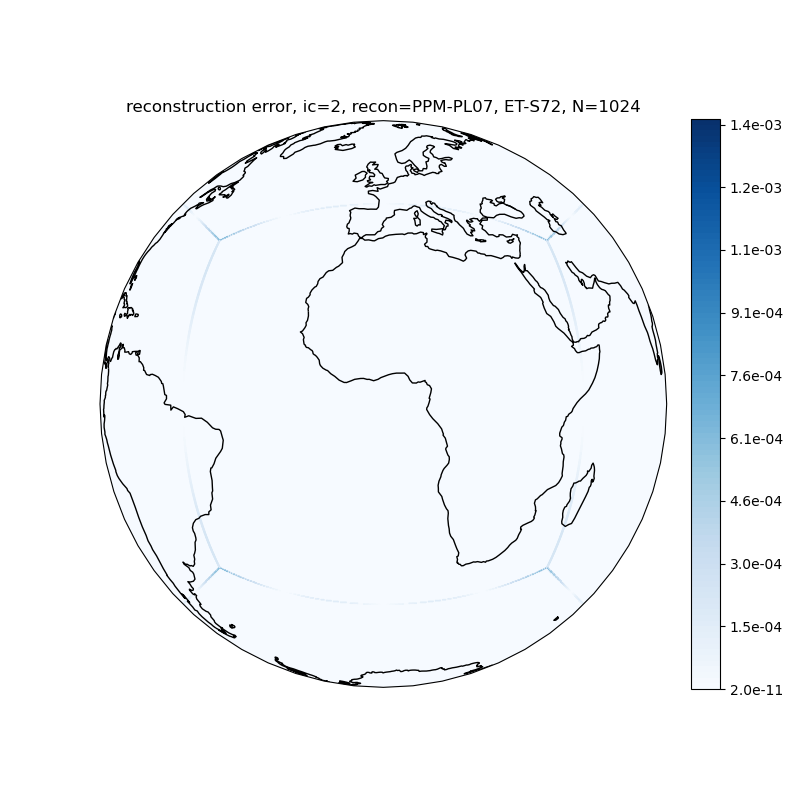
\includegraphics[width=1\linewidth]{gnomonic_equiangular_cs_1024_recon_q_ic_2_reconPPM-PL07_etET-S72_sphere}
		\caption{ET-S72.\label{chp4-exp4-a}}
	\end{subfigure}
	\begin{subfigure}{0.3\textwidth}
		\centering
		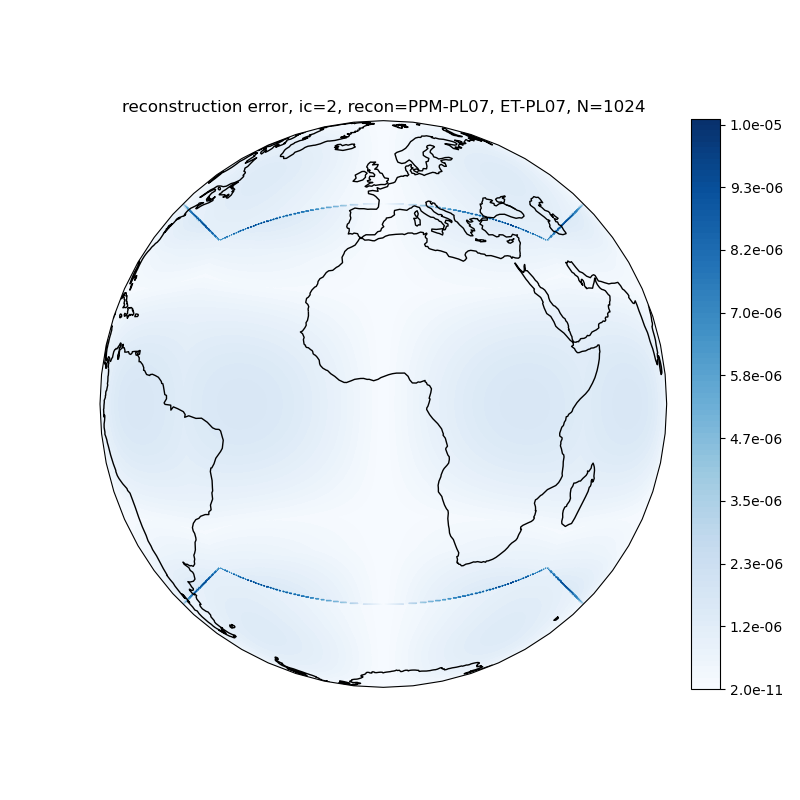
\includegraphics[width=1\linewidth]{gnomonic_equiangular_cs_1024_recon_q_ic_2_reconPPM-PL07_etET-PL07_sphere}
		\caption{ET-PL07.\label{chp4-exp4-b}}
	\end{subfigure}
	\begin{subfigure}{0.3\textwidth}
	\centering
	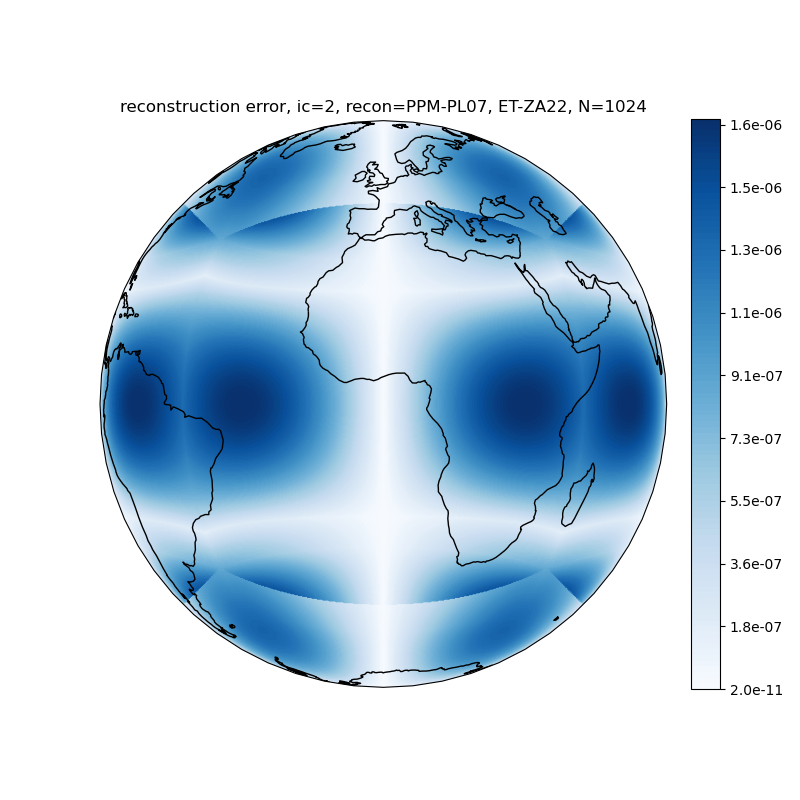
\includegraphics[width=1\linewidth]{gnomonic_equiangular_cs_1024_recon_q_ic_2_reconPPM-PL07_etET-ZA22_sphere}
	\caption{ET-ZA22.\label{chp4-exp4-c}}
\end{subfigure}
	\caption{Error for the edge midpoint values considering the trigonometric function (Equation \eqref{chp4-ic2})
	with edges treatment schemes ET-S72 (a), ET-PL07 (b) and ET-ZA22 for the cubed-sphere with $N=1024$ using the reconstruction PPM-PL07.\label{chp4-exp4}}
\end{figure}
\begin{figure}[!ht]
	\centering
	\begin{subfigure}{0.3\textwidth}
		\centering
		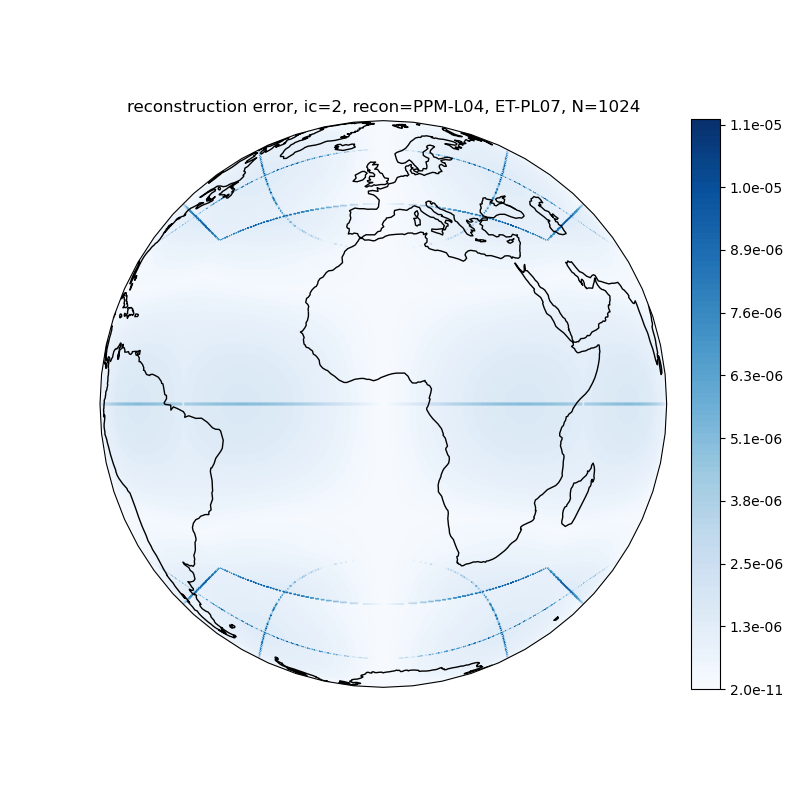
\includegraphics[width=1\linewidth]{gnomonic_equiangular_cs_1024_recon_q_ic_2_reconPPM-L04_etET-PL07_sphere}
		\caption{ET-S72.\label{chp4-exp5-a}}
	\end{subfigure}
	\begin{subfigure}{0.3\textwidth}
		\centering
		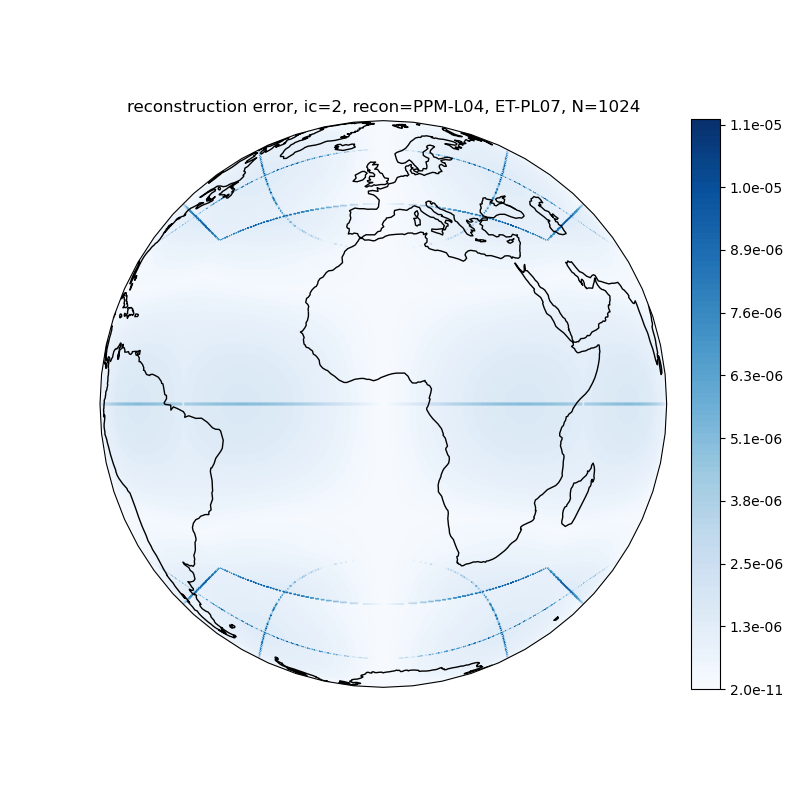
\includegraphics[width=1\linewidth]{gnomonic_equiangular_cs_1024_recon_q_ic_2_reconPPM-L04_etET-PL07_sphere}
		\caption{ET-PL07.\label{chp4-exp5-b}}
	\end{subfigure}
	\begin{subfigure}{0.3\textwidth}
		\centering
		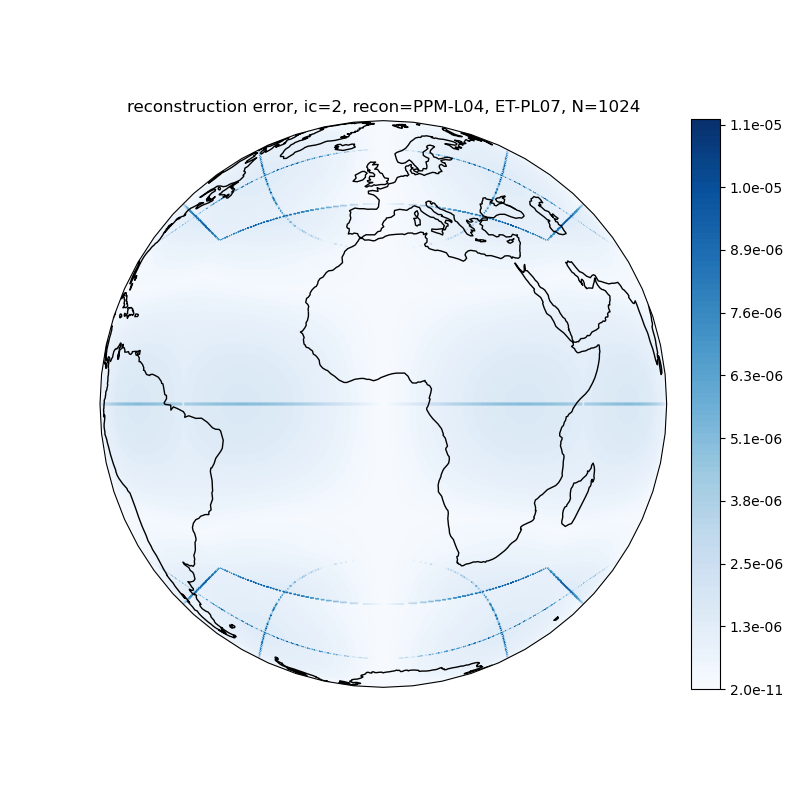
\includegraphics[width=1\linewidth]{gnomonic_equiangular_cs_1024_recon_q_ic_2_reconPPM-L04_etET-PL07_sphere}
		\caption{ET-ZA22.\label{chp4-exp5-c}}
	\end{subfigure}
	\caption{As Figure in \ref{chp4-exp4} but using the PPM-L04 scheme.\label{chp4-exp5}}
\end{figure}

\newpage
\section{Concluding remarks}
\label{cs-conc}

